\documentclass[8pt, a4paper, landscape, fleqn]{scrartcl}
\usepackage[utf8]{inputenc}
\usepackage[ngerman]{babel}

%Layout
\usepackage{multicol, geometry, xcolor}
\geometry{margin=1cm}
%\titlespacing{\section}{0pt}{3pt}{1pt}
%\titlespacing{\subsection}{0pt}{3pt}{1pt}
%\titlespacing{\subsubsection}{0pt}{3pt}{1pt}
\parindent 0pt
\pagestyle{empty}

\newlength{\breite}
\setlength{\breite}{0.5pt}
\setlength{\columnseprule}{\breite}

\usepackage{graphicx}
\usepackage{enumitem}
\usepackage{svg}


%Seitenzahl
\usepackage{fancyhdr}
\pagestyle{fancy}
\fancyhf{}
\rhead{\sffamily\textbf\thepage}
\renewcommand{\headrulewidth}{0pt}

%Mathematik-Pakete
\usepackage{amsmath, amstext, amssymb, mathtools, esint, polynom}
\usepackage{bm}
\allowdisplaybreaks %Seitenumbruch in align-Umgebung erlauben



%Definition der Umgebung "example"
\newenvironment {example}
				{\begin{itshape} \begin{small}}
				{\end{small} \end{itshape}}
%Definition der Umgebung "annotation"		
\newenvironment {annotation}[1]
				{\begin{itshape} \begin{small} \textbf{#1} \begin{itemize}}
				{\end{itemize} \end{small} \end{itshape}}
%Definition der Umgebung "eq"
\newenvironment {eq}
				{\begin{equation*}}
				{\end{equation*}}

% define some colors
% ETH corporate design colors
\definecolor{subsection}{RGB}{191, 83, 79} % ETH 7 80%
\definecolor{section}{RGB}{168, 50, 45} % ETH 7 100%
\definecolor{titletext}{RGB}{255,255,255}



% section color box
\setkomafont{section}{\mysection}
\newcommand{\mysection}[1]{%
	\Large\sf%
	\setlength{\fboxsep}{0cm}%already boxed
	\colorbox{section}{%
		\begin{minipage}{\linewidth}%
			\vspace*{2pt}%Space before
			\leftskip2pt %Space left
			\rightskip\leftskip %Space right
			{\color{titletext} #1}
			\vspace*{1pt}%Space after
		\end{minipage}%
}}
% subsection color box
\setkomafont{subsection}{\mysubsection}
\newcommand{\mysubsection}[1]{%
	\Large\sf%
	\setlength{\fboxsep}{0cm}%already boxed
	\colorbox{subsection}{%
		\begin{minipage}{\linewidth}%
			\vspace*{2pt}%Space before
			\leftskip2pt %Space left
			\rightskip\leftskip %Space right
			{\color{titletext} #1}
			\vspace*{1pt}%Space after
		\end{minipage}%
}}

% Symbol commands
\def\R{\mathbb{R}}
\def\Z{\mathbb{Z}}
\def\N{\mathbb{N}}
\def\C{\mathbb{C}}
\def\d{\text{d}}
\def\Re{\text{Re}}
\def\Im{\text{Im}}
\def\Res{\text{Res}}
\def\Arg{\text{Arg}}
\def\Log{\text{Log}}
\definecolor{ethblue}{RGB}{18, 105, 176}
\newcommand{\blue}[1]{\textcolor{ethblue}{#1}}
\def\F{\mathcal{F}}
\def\FI{\mathcal{F}^{-1}}

				
\providecommand{\diff}{\mathop{} \! \mathrm{d}}

\title{Komplexe Analysis}
\subtitle{FS21 ETH Zürich \\Prof. A. Iozzi}
\author{Robin Sieber \\ rosieber@ethz.ch}
\date{\today}
 
\begin{document}
	\begin{multicols*}{3}
		\maketitle
		\section{Grundlagen}
		    \subsection{Quantoren}
		    	\vspace{-8pt}
				\begin{align*}
					&\forall \hspace{10pt} \text{für alle}\\
					&\exists \hspace{10pt} \text{es existiert ein}\\
					&\nexists \hspace{11pt} \text{es existiert kein}\\
					&\exists! \hspace{9pt} \text{es existiert genau ein}
				\end{align*}
			\subsection{Logik}
		        \begin{tabular}{|c|c|}
					\hline
					$\lnot A$ & nicht A \\
					\hline
					$A \land B$ &  A und B\\
					\hline
					$A\lor B$ & A oder B (incl. OR)\\
					\hline
					$A\Rightarrow B$ & A impliziert B \\
					\hline
					$A\Leftrightarrow B$ & A gilt genau dann wenn B \\
					\hline 
				\end{tabular}\\
				$(A \Rightarrow B) \equiv (\lnot B \Rightarrow \lnot A) \equiv (\lnot A \lor B)$
		    \subsection{Mengenoperationen}
		        	\begin{tabular}{|c|c|}
						\hline
						$x\in A$ & Element von\\
						\hline
						$A\subset B$ &  Teilmenge von\\
						\hline
						$A\cap B$ & Durchschnitt\\
						\hline
						$A\cup B$ & Vereinigt \\
						\hline
						$A\cap B = \emptyset$ & Disj. Vereinigung \\
						\hline
						$A \setminus B$ & Differenz \\
						\hline
						$A \Delta B := (A \setminus B)\cup (B \setminus A)$ & Sym. Differenz \\
						\hline
						$A^c$ & Komplementär \\
						\hline
						$[a,b]$ & Abgeschl. (inkl.) \\
						\hline
						$(a,b), \ ]a,b[$ & Offen (exkl.) \\
						\hline
					\end{tabular}\\
			\subsection{Komplexe Zahlen}
			\begin{itemize}
			    \item $z = x + iy = re^{i\varphi}$
			    \item $\overline{z} = x - iy = re^{-i\varphi}$
			    \item $i^2 = -1,\ i^3 = -i,\ i^4 = 1, \ (-i)^2 = -1,\ (-i)^3 = i,\ (-i)^4 = 1$ 
			    \item $i^{-1} = \frac{1}{i} = -i$
			    \item $z \cdot z' = xx' - yy' + i(x'y + y'x) = rr' \cdot e^{i(\varphi + \varphi')}$
			    \item $\frac{1}{z} = \frac{\overline{z}}{z\overline{z}} = \frac{x-iy}{x^2+y^2}$
			    \item $e^z = e^{x+iy} = e^x(\cos(y)+i\sin(y))$
			    \item $z^n = (r\cdot e^{i\varphi})^n = r^n \cdot e^{i\varphi n}$
			    \item $\Re(z) = x = \frac{z+\overline{z}}{2},\hspace{10pt} \Im(z) = y = \frac{z-\overline{z}}{2i}$
			    \item $\overline{z_1 + z_2} = \overline{z_1} + \overline{z_2}, \hspace{10pt} \overline{z_1 \cdot z_2} = \overline{z_1} \cdot \overline{z_2}$
			    \item $\vert z_1 \cdot z_2\vert = \vert z_1 \vert \cdot \vert z_2 \vert$
			    \item Dreiecksungleichung: $\vert z_1 + z_2 \vert \leq \vert z_1 \vert + \vert z_2 \vert$
			    \item $\arg(z) = \{\varphi + 2\pi k \ \vert \ k \in \Z \}, \hspace{10pt} \Arg(z) = \varphi$ (Hauptwert)
			    \item $\Arg(\varphi) = \begin{cases}
			    \arctan(y/x) &z \text{ im 1. oder 4. Quadranten} \\
			    \arctan(y/x)+\pi &z \text{ im 2. Quadranten} \\
			    \arctan(y/x)-\pi &z \text{ im 3. Quadranten}
			    \end{cases}$ \\
			    \item $n$-te Wurzel: $\sqrt[n]{z} = w_k = r^{\frac{1}{n}}e^{i\left(\frac{\varphi}{n}+\frac{2k\pi}{n}\right)}$ für $k \in \{0,\dots, n-1\}$
			    \item $\log(z) = \log(|z|) + i \arg(z)$ (nicht eindeutig!)
			    \item Hauptwert: $\Log(z) := \log(|z|)+ i \Arg(z)$ stetig für $\C\setminus\R^-$ (log-Gesetze gelten nicht)
			\end{itemize}
		\section{Stetigkeit, Differenzierbarkeit \& Holomorphie}
		\subsection{Stetigkeit}
		$f$ ist \blue{stetig} $\Leftrightarrow \lim_{z \to z_0} f(z) = f(z_0)$ \vspace{5pt}
	
		\begin{example}
		    \textbf{Bemerkung.}
		    Der Limes muss für jede Richtung in der $\C$-Ebene gleich sein. Gegenbeweis einfach per Counter-Example, wenn 2 Richtungen nicht denselben Grenzwert haben. Mögliche Richtungen zum Überprüfen: $x = 0, \ y = 0, \ y = x, \ y = x^2$ etc.
		\end{example} \\
	    
	    Verknüpfungen und Linearkombinationen stetiger Funktionen sind stetig.
	
	    \subsection{Differenzierbarkeit}
	    $f$ ist \blue{$\C$-differenzierbar} in $z_0 \Leftrightarrow \lim_{z \to z_0} \frac{f(z)-f(z_0)}{z-z_0} = f'(z_0) = \frac{\d}{\d z}f(z_0)$ existiert. \\
	    
	    \begin{example}
		    \textbf{Bemerkung.}
		    $|z|, \Re(z), \Im(z), \overline{z}$ sind in keinem Punkt $\C$-diffbar. $|z|^2$ ist einzig an der Stelle 0 diffbar, aber nicht holomorph, weil nicht in einer Umgebung um 0 diffbar (durch obige $\lim$-Def. überprüfen).
		\end{example} \\
		
		Es ist möglich, dass eine Funktion stetige partielle Ableitungen besitzt, aber trotzdem nicht $\C$-differenzierbar ist. 
		
		
		\subsection{Holomorphie}
		Eine Funktion $f: U \to \C$ heisst \blue{holomorph auf $U$}, falls sie auf ganz $U$ $\C$-differenzierbar ist. $f$ heisst \blue{holomorph in $z_0$}, falls sie in einer offenen Menge um $z_0$ holomorph ist. $\Rightarrow$ Holomorphie in einem einzigen Punkt ist per Definition nicht möglich. \\
		
		Sei $f: U \to \C$ mit $f(z) = f(x, y) = u(x, y) + i v(x, y)$ holomorph. Dann existieren die partiellen Ableitungen $u_x, u_y, v_x, v_y$ ($\frac{\partial u}{\partial x} = u_x$) und die \blue{Cauchy-Riemann Gleichungen (CRG)} werden erfüllt:
% 		\begin{align*}
% 		    u_x(x, y) &= v_y(x, y) &u_y(x, y) = -v_x(x, y) \\
% 		    f'(z) &= u_x(z)+iv_x(z) = -iu_y(z)+v_y(z) &= \frac{\partial f}{\partial x}(z) = -i \frac{\partial f}{\partial y}(z)
% 		\end{align*}
		\begin{multicols}{2}
    		\begin{itemize}
    			\item $ u_x(x, y) = v_y(x, y)$
    			\item $u_y(x, y) = -v_x(x, y)$
    		\end{itemize}
    	    \end{multicols}
    	    \begin{itemize}
		        \item $f'(z) = u_x(z)+iv_x(z) = -iu_y(z)+v_y(z) = \frac{\partial f}{\partial x}(z) = -i \frac{\partial f}{\partial y}(z)$
		    \end{itemize}
			\setlength{\columnseprule}{0.5pt}
		%\vspace{-1.3cm}
% 		\begin{align*}
% 		    f'(z) = u_x(z)+iv_x(z) = -iu_y(z)+v_y(z) = \frac{\partial f}{\partial x}(z) = -i \frac{\partial f}{\partial y}(z)
% 		\end{align*} \\
		
		Bedingung für Holomorphie: \\ Sei $f: U \to \C, z_0 \in U$. Falls $u_x, u_y, v_x, v_y$ \dots
		\begin{enumerate}
		    \item  in einer \textit{offenen} Menge um $z_0$ existieren, und
		    \item  in $z_0$ stetig sind und die CRG erfüllen
		\end{enumerate} Dann existiert $f'(z_0)$, d.h. $f$ ist $\C$-differenzierbar.  
		
		\vspace{5pt}
		Ausserdem gilt für $f$ holomorph: 
		\begin{itemize}
		    \item $\frac{\partial^2 u}{\partial x^2} + \frac{\partial^2 u}{\partial y^2} = \frac{\partial^2 v}{\partial x^2} + \frac{\partial^2 v}{\partial y^2} = 0$
		    \item Falls $f$ holomorph, sind auch alle Ableitungen $f^{(n)}$ holomorph.
		    \item $\vert f(z) \vert$ konstant $\Rightarrow f(z)$ konstant
		    \item $|f(z)|$ kann im Inneren einer Menge kein Maximum annehmen. Ausser $f(z)$ ist konstant. ($\rightarrow$ vgl. Max-Mod., Kap. \ref{sec:max-mod})
		\end{itemize}
        Insbesondere sind Polynome, $\exp, \sin, \cos, \sinh, \cosh$ holomorph auf $\C$.
        
        \section{Integrale}
        \subsection{Kurvenintegrale}
        \subsubsection{Stammfunktionen}
        Eine Menge $U$ heisst \blue{wegzusammenhängend (wzh.)}, falls es für zwei bel. Punkte $z_1, z_2 \in U$ einen Pfad gibt, der die zwei Punkte verbindet. \\
        
        Sei $U$ wzh. und offen, $f: U\to\C$ stetig. Dann sind folgende Aussagen äquivalent. 
        \begin{enumerate}
            \item Für jede geschlossene Kurve $\gamma : [a, b]\to U$ gilt $\int_\gamma f(z)\d z = 0$
            \item Das Kurvenintegral $\int_\gamma f(z)\d z$ ist unabhängig vom Pfad
            \item Es gibt eine $\C$-diffbare Funktion $F : U\to\C$ mit $F'(z) = f(z)$
        \end{enumerate}
        Falls eine (und deshalb jede) der Aussagen gilt, heisst $F$ Stammfunktion von $f$ und ist bis auf eine Konstante eindeutig. $$\int_\gamma f(z)\d z = F(\gamma(b)) - F(\gamma(a))$$
        
        
        \subsubsection{Kurvenintegral}
        Ein \blue{Pfad} ist eine stetige Abbildung $\gamma : [a, b]\to\C$. Ein Pfad ist einfach, wenn er keine Selbstschnitte hat und geschlossen, falls $\gamma(a) = \gamma(b)$ gilt. \\
        
        Sei $U\subset \C$ offen, $f:U\to\C$ stetig und sei $\gamma : [a, b] \to U$ diffbar. $$ \int_\gamma f(z) \d z := \int_a^b f(\gamma(t))\cdot \dot{\gamma}(t)\d t $$
        bzw. auch $= \int_a^b \Re(f(\gamma(t))\cdot\dot{\gamma}(t))\d t + i \int_a^b \Im(f(\gamma(t))\cdot\dot{\gamma}(t))\d t$ \\
        $\gamma$ darf an endlich vielen Stellen nur stetig und nicht diffbar sein. \\
        
        Es gelten folgende Eigenschaften:
    	\begin{itemize}[leftmargin=1cm]
          \item[(KI1)] (Linearität) Für $\alpha, \beta \in\C$ gilt $$\int_\gamma [\alpha f(z) + \beta g(z)]\d z = \alpha \int_\gamma f(z)\d z + \beta \int_\gamma g(z)\d z$$
          \item[(KI2)] Sei $\gamma, \delta : [0, 1]\to\C$, $\delta(t) := \gamma(1-t)$. Dann ist $$\int_\gamma f(z)\d z = -\int_\delta f(z)\d z $$
          \item[(KI3)] Sei $\delta : [0, 1]\to\C$ mit $\gamma(1) = \delta(0)$ mit der Verkettung $$(\gamma * \delta)(t) := \begin{cases}
          \gamma(2t) & 0 \leq t \leq 1/2 \\ \delta(2t-1) & 1/2 \leq t \leq 1
          \end{cases} $$ $$ \int_{\gamma*\delta}f(z)\d z = \int_\gamma f(z)\d z + \int_\delta f(z) \d z$$
          \item[(KI4)] (Unabhängigkeit der Parametrisierung) Sei $\delta$ eine andere Parametrisierung des Bildes von $\gamma$. Dann gilt $$ \int_\gamma f(z)\d z = \int_\delta f(z)\d z $$
          \item[(KI5)] Sei $U$ wzh. $$\left\vert \int_a^b f(\gamma(t)) \cdot \dot{\gamma}(t) \d t \right\vert \leq \int_a^b \vert f(\gamma(t)) \cdot \dot{\gamma}(t)\vert \d t$$
          \item[(KI6)] Sei $L = \int_a^b \vert \dot{\gamma}(t)\vert\d t$ die Länge von $\gamma$. Wenn $\vert f(z) \vert \leq M\ \forall z \in U$, dann folgt $$ \left\vert \int_\gamma f(z)\d z \right\vert \leq M\cdot L $$
          %\item[(KI7)] \blue{vgl. S. 50 Skript} % halte ich für unwichtig
        \end{itemize}
        
        
        
        \subsection{Cauchy'scher Integralsatz}
        \subsubsection{Einfach zusammenhängend}
        \begin{itemize}
            \item Eine Menge $U$ ist \blue{einfach zusammenhängend (ezh.)} $\Leftrightarrow$ wzh. $\land$ bel. zwei Pfade von $a$ nach $b$ sind homotop (``deformierbar'')
            \item $U \subset \C$ ezh. und offen, $f: U \to \C$ holomorph $\Rightarrow f$ besitzt Stammfunktion (Achtung: $\not\Leftarrow$)
        \end{itemize}
        \subsubsection{Cauchy Integralformel}
        $z_0 \in U \subset \C$ ezh. und offen, $f: U \to \C$ holomorph, $\gamma : [a, b] \to \C \setminus \{z_0\}$ umläuft $z_0$ einmal in positiver Richtung, dann gilt: $$ f(z_0) = \frac{1}{2\pi i}\int_\gamma \frac{f(z)}{z-z_0} \d z \ \text{ und}$$ $$ f^{(n)}(z_0) = \frac{n!}{2\pi i}\int_\gamma \frac{f(z)}{(z-z_0)^{n+1}}\d z$$ \\
        \begin{example}
		    \textbf{Bemerkung.}
		    Der Integrand muss nicht holomorph sein, nur $f$ selbst. Ansonsten wäre das Integral sowieso 0. CIF funktioniert nur für Pole, für andere Singularitäten $\rightarrow$ Residuensatz
		\end{example}
		  
        \subsection{Residuensatz}
	    Sei $\gamma$ positiv orientiert und geschlossen. 
	    $$ \int_\gamma f(z) \d z = 2\pi i \cdot \sum_i W(\gamma, z_i) \cdot \Res(f, z_i) $$ \\
	    Windungszahl $W(\gamma, z) = $ \#Umrundungen von $\gamma$ um $z$ im GUZ
        
        \subsubsection{Arten von Singularitäten $\to$ vgl. \ref{sec:singularity}}

	    \subsubsection{Residuenberechnung an Polstellen}
	    \begin{enumerate}
	        \item Ordnung: $\Res(f, z_0) = \lim_{z \to z_0} (z-z_0)f(z)$ 
	        \item[$n$.] Ordnung: $\Res(f, z_0) = \mathbf{\frac{1}{(n-1)!}} \lim_{z\to z_0}\frac{\d^{n-1}}{\d z^{n-1}}((z-z_0)^nf(z))$
	        \item[] Res($f,z_0) = \frac{p(z_0)}{q'(z_0)}$ für $f(z) = \frac{p(z)}{q(z)}$ und $p,q$ analytisch, wobei $z_0$ eine einfache Nullstelle von $q$ ist.
	    \end{enumerate}
	    Wenn $z_0$ eine Singularität $n$-ter Ordnung ist, muss $f(z)\cdot(z-z_0)^n$ an der Stelle $z_0 \neq 0$ sein. Falls dies nicht der Fall ist, muss das Residuum mittels Laurentreihe berechnet werden.\\Bsp.: $\sinh(z)/z^4 \Rightarrow g(z) = z^4f(z) = \sinh(z)$ mit $g(0) = 0 \Rightarrow$ mit Laurentreihe erhält man $\Res(f, 0) = 1/3!$ 
	    
	    
	    \subsubsection{Residuenberechnung an anderen Singularitäten}
	    $\rightarrow$ Funktion in Laurentreihe entwickeln, dann Koeffizient $c_{-1}$ ablesen \\
	    
	    \subsection{Uneigentliche Integrale}
	    Der Limes $$ \lim_{R\to\infty}\int_{-R}^R f(z) \d z =: P.V. \int_{-\infty}^\infty f(z) \d z$$ wird als \blue{Cauchy-Hauptwert (P.V. = principal value)} des Integrals $\int_{-\infty}^\infty f(z) \d z$ bezeichnet.\\
	    Definition des ``normalen'' uneigentlichen Integrals: $$ \int_{-\infty}^\infty f(x) \d x = \lim_{R\to\infty} \int_{-R}^0 f(x) \d x + \lim_{R\to\infty} \int_0^R f(x) \d x$$
	    Falls beide Integrale auf der rechten Seite existieren, existiert auch der $P.V.$, umgekehrt gilt die Implikation nicht! Bsp.: $P.V. \int_{-\infty}^\infty x \d x = 0$, aber $\int_{-\infty}^\infty x \d x = -\infty + \infty$ (unbestimmt)\\
	    \textit{Für \textbf{gerade} Funktionen ist der Cauchy-Hauptwert = uneigentliches Integral.}
	    
	    
	    \subsubsection{Uneigentliche Integrale mit dem Residuensatz berechnen}
	    Ziel: Integral mit dem Residuensatz berechnen über dem Pfad $\gamma(t) = \gamma_1(t) * \gamma_2 (t)$ mit $\gamma_1(t) = -R + 2Rt \ (t\in [0, 1])$ und $\gamma_2(t) = Re^{i\pi t}\ (t\in [0, 1])$
	    Es gilt $$P.V. \int_{-\infty}^\infty f(z) \d z = 2\pi i \sum_{\Im(z_k)>0} \Res(f, z_k), $$ falls $\int_{\gamma_2} f(z) \d z = 0$. Dies gilt genau dann, wenn ($f: \C\to\C$): 
	    \begin{enumerate}
	        \item $f(z) := \frac{p(z)}{q(z)}h(z)$ mit $p, q$ Polynomen
	        \item $\deg(q) \geq \deg(p)+2$
	        \item $|h(z)| < C$ auf $\{z \ | \ \Im(z) \geq 0\}$ (beschränkt)
	        \item $q(z)$ hat keine Nullstelle auf der $x$-Achse
	    \end{enumerate}
	    \begin{example}
	        \textbf{Bemerkung. } Das Ganze gilt auch für die untere Hälfte des Koordinatensystems. Die Formel und Pfade müsssen einfach entsprechend angepasst werden. 
	    \end{example}
	    
	    

        \section{Reihenentwicklung}
	    \subsection{Taylorreihe}
	    Sei $f : B(z_0, R_0) \to \C$ eine holomorphe Funktion und $R_0 > 0$. Dann konvergiert folgende Reihe $\forall z \in B(z_0, R_0)$: 
	    $$ f(z) = \sum_{n = 0}^\infty \frac{1}{n!}f^{(n)}(z_0)(z-z_0)^n$$ 
	    
	    \subsection{Laurentreihe}
	    Sei $f$ holomorph auf dem Kreisring $R_1 < \vert z - z_0 \vert < R_2$. Dann gilt folgende Reihenentwicklung: 
	    $$ f(z) = \sum_{n = 0}^\infty a_n(z-z_0)^n + \sum_{n=1}^\infty b_n \frac{1}{(z-z_0)^n} = \sum_{n = -\infty}^\infty c_n (z-z_0)^n$$ mit $a_n = \frac{1}{2\pi i}\int_\gamma \frac{f(z)}{(z-z_0)^{n+1}}\d z \ $ $\tiny{(n = 0, 1, 2, ...)}$ und $b_n = \frac{1}{2\pi i} \int_\gamma \frac{f(z)}{(z-z_0)^{-n+1}}\d z \ $ $\tiny{(n = 1, 2, ...)}$, bzw $c_n = \frac{1}{2\pi i}\int_\gamma \frac{f(z)}{(z-z_0)^{n+1}}\d z \ (n = 0, \pm 1, \pm 2, ...)$ wobei $\gamma$ ein geschlossener Pfad im Kreisring ist (im GUZ). \\
	    Spezialfall: $c_{-1} = \frac{1}{2\pi i}\int_\gamma f(z)\d z$
	    
	    \subsection{Singularitäten}
	    \label{sec:singularity}
        Sei $ z_0 \in U, f: U\setminus\{z_0\} \to \C$ holomorph. Falls $f$ in $z_0$ nicht definiert oder analytisch ist, heisst $z_0$ eine \blue{Singularität}. Der Punkt $z_0$ ist eine \blue{isolierte Singularität} von $f$, falls es ein $\epsilon > 0$ gibt, so dass $f$ keine weitere Singularität in der Scheibe $B(z_0, \epsilon)$ hat. \\
        \begin{example}
            \textbf{Beispiel. } $\sin\frac{1}{z}$ hat im Ursprung eine isolierte Singularität. $\frac{1}{\sin\frac{1}{z}}$ hat im Ursprung eine Singularität, die nicht isoliert ist (Singularitäten bei $1/(n\pi)$, es lässt sich also keine Scheibe um 0 finden, in der es keine Singularität hat. 
        \end{example}
	    \subsubsection{Arten von Singularitäten}
	    Seien $U \subset \C$ offen, $z_0 \in U$ und $f$ holomorph auf $U \setminus \{z_0\}$. Schreiben wir $f(z) = \sum_{n=-\infty}^\infty c_n(z-z_0)^n$ für jedes $z \in B(z_0, R)\setminus\{z_0\}$ für $R>0$, so definiert man: 
	    \begin{enumerate}
	        \item $z_0$ ist eine \blue{wesentliche Singularität}, falls $c_n \neq 0$ für unendlich viele $n<0$
	        \item $z_0$ ist ein \blue{Pol der Ordnung $m\geq 1$}, falls $c_{-m} \neq 0$ und $c_n = 0$ für alle $n< -m$. Falls $m=1$, heisst $z_0$ einfacher Pol.
	        \item $z_0$ ist eine \blue{hebbare Singularität}, falls $c_n = 0$ für alle $n < 0$
	        \item $z_0$ ist eine \blue{Nullstelle der Ordnung $m\geq 0$}, falls $c_m\neq 0$ und $c_n = 0$ für alle $n<m$  
	    \end{enumerate}
	    
	    \textbf{Lemma: } Sei $f : U \to \C$ holomorph an der Stelle $z_0\in U$. $f$ hat an der Stelle $z_0$ eine NS der Ordnung $m \Leftrightarrow \exists g: U\to \C$ holomorph mit $f(z) = (z-z_0)^mg(z)$ und $g(z_0) \neq 0$. \\
	    \textbf{Korollar: } Seien $p, q$ holomorph an der Stelle $z_0$ mit $p(z_0) \neq 0$ und sei $z_0$ eine Nullstelle der Ordnung $m$ für $q$. Dann ist $z_0$ ein Pol der Ordnung $m$ für $\frac{p(z)}{q(z)}$.\\
	    \textbf{Lemma: } Sei $f:B(z_0, \epsilon) \to \C$ holomorph und sei $f(z_0) = 0$. Entweder ist $f(z) \equiv 0$ oder $z_0$ ist eine isolierte NS.\\
	    \textbf{Satz: } Sei $f: U\to\C$ holomorph und $U$ wzh. Falls $f(z) \equiv 0$ auf einer offenen Menge oder auf einer Geradenstrecke, ist $f(z) \equiv 0$ auf $U$.\\
	    \textbf{Korollar: } Sei $U$ offen, $f, g: U\to\C$ holomorph. Falls $f(z) = g(z)$ auf einer offenen Menge oder einer Geradenstrecke in $U$, dann gilt $f(z) \equiv g(z)$. \textit{Gilt nicht für reellwertige Funktionen!}
	    
	    
	    
	    \subsubsection{Satz von Picard}
	    Sei $z_0$ eine wesentliche Singularität von $f$ holomorph. Für jedes $\epsilon > 0$ nimmt $f(z)$ auf $B(z_0, \epsilon)$ alle komplexen Werte mit höchstens einer Ausnahme unendlich oft an. 
	
		
		\subsection{Fourierreihen}
		\subsubsection{Periodizität}
		Sei $f: \R \to \C$. Falls es $p\in\R$ gibt, so dass $$f(t+p) = f(t) \ \forall t\in\R$$ heisst $f$ \blue{periodisch} und $p$ heisst die Periode von $f$. Die Frequenz von $f$ ist $1/p$. Die kleinste Periode heisst Fundamentalperiode.\\
		Sei $f$ eine Funktion, die auf einem endlichen Intervall definiert ist. Man kann $f$ periodisch fortsetzen: z.B. $$f(t) := \begin{cases}
		1 & t\in \ ]0, \frac{L}{2}]\\ 0 & t\in \ ]\frac{L}{2}, L[ \end{cases} $$ Man kann als $f$ als $L$-periodische Funktion fortsetzen oder als $2L$-periodische Funktion, wobei $f$ entweder als gerade oder ungerade Funktion fortgesetzt wird.
		
		\subsubsection{Trigonometrisches Polynom}
		Ein trig. Polynom des $N$-ten Grades ist eine endliche Linearkombination der Form $$ \frac{a_0}{2}+\sum_{n=1}^N\left(a_n \cos\left(\frac{n\pi}{L}t\right)+b_n \sin\left(\frac{n\pi}{L}t\right)\right) \Leftrightarrow \sum_{n = -N}^N c_n e^{i\frac{n\pi}{L}t}$$
		Es gelten folgende Orthogonalitätsrelationen ($n, m \in \N_0$):
		\begin{enumerate}
		    \item $$ \int_{-L}^L \cos\left(\frac{n\pi}{L}t\right)\cos\left(\frac{m\pi}{L}t\right)\d t = \begin{cases}
		    0 & n\neq m \\ L & n = m \neq 0 \\ 2L & n = m = 0 \end{cases} $$
		    \item $$ \int_{-L}^L \sin\left(\frac{n\pi}{L}t\right)\sin\left(\frac{m\pi}{L}t\right)\d t = \begin{cases}
		    0 & n\neq m \\ L & n = m \neq 0 \end{cases} $$
		    \item $$ \int_{-L}^L \cos\left(\frac{n\pi}{L}t\right)\sin\left(\frac{m\pi}{L}t\right)\d t = 0 \ \forall n, m$$
		\end{enumerate}
		
		\subsubsection{Fourierreihe}
		Sei $f$ eine $2L$-periodische Funktion. Es gilt: $$ f(t) = \frac{a_0}{2}+\sum_{n=1}^\infty \left(a_n \cos\left(\frac{n\pi}{L}t\right)+b_n \sin\left(\frac{n\pi}{L}t\right)\right) = \sum_{n = -\infty}^\infty c_n e^{i\frac{n\pi}{L}t}$$
		mit $$ a_m = \frac{1}{L}\int_{-L}^L f(t)\cos\left(\frac{m\pi}{L}t\right)\d t \text{, falls } m \geq 0$$
		$$ b_m = \frac{1}{L}\int_{-L}^L f(t)\sin\left(\frac{m\pi}{L}t\right)\d t \text{, falls } m > 0$$
		$$ c_m = \frac{1}{2L}\int_{-L}^L f(t)e^{i\frac{m\pi}{L}t}\d t \text{, falls } m \in\Z$$
		Ausserdem gilt folgendes: 
		\setlength{\columnseprule}{0pt}
		\begin{multicols}{2}
			\begin{itemize}
				\item $c_n = \frac{1}{2}(a_n - i b_n)$
				\item $a_n = c_n + c_{-n}$
				\item $a_n \equiv 0$, falls $f$ ungerade
				\item $c_{-n} = \frac{1}{2}(a_n + i b_n)$
				\item $b_n = i(c_n - c_{-n})$
				\item $b_n \equiv 0$, falls $f$ gerade
			\end{itemize}
		\end{multicols}
		\setlength{\columnseprule}{0.5pt}
		An einer \blue{Sprungstelle} von $f$ ist der zugehörige der Wert der FR $\frac{1}{2}\left(\lim_{t\to t_0^-}f(t) + \lim_{t\to t_0^+} f(t)\right)$ \\
		
		\textbf{Satz: } Sei $f$ eine $2L$-periodische Funktion auf $[-L, L]$, die stückweise stetig ist und die linke und rechte Ableitung an jedem Punkt in $[-L, L]$ hat. Dann besitzt $f$ genau eine FR, durch welche sie für alle Werte dargestellt wird (\blue{Eindeutigkeit der FR}).
		
		%\subsubsection{\blue{Kap. 4.1.7, 4.1.8 relevant?}}
		\subsubsection{Satz von Parseval}
		Das trig. Polynom des Grades $N$, das am besten eine $2\pi$-periodische Funktion $f$ auf dem Intervall $[-\pi, \pi]$ approximiert (kleinster quadr. Fehler), ist die partielle Summe $s_N$ der Fourier-Reihenentwicklung von $f$. Der kleinste Wert $E^*_N(f)$ von dem quadratischen Fehler ist $$ E^*_N (f) = \frac{1}{2\pi}\int_{-\pi}^{\pi} |f(t)|^2 \d t - \sum_{n=-N}^N |c_n|^2 $$ und $E^*_N (f)$ ist monoton abnehmend mit zunehmendem N. \\
		Daraus folgt die Parseval'sche Identität $$ \sum_{n=-\infty}^\infty |c_n|^2 = \frac{1}{2\pi} \int_{-\pi}^\pi |f(t)|^2 \d t$$ bzw. in reeller Form: $\frac{1}{2}\left(a_0^2/2 + \sum_{n=1}^\infty (a_n^2+b_n^2)\right)$
		
		\subsubsection{Prüfungsaufgabe}
		Wenn man an der Prüfung eine Reihe berechnen muss:
		\begin{enumerate}
		    \item $n$ kommt in der FR mit derselben Potenz vor wie in der gesuchten Reihe $\Rightarrow t$ geschickt wählen und Reihen vergleichen
		    \item $n$ kommt irgendwie quadratisch vor $\Rightarrow$ Parseval anwenden und Integral berechnen
		\end{enumerate}
		
		\section{Transformationen}
		\subsection{Fourier-Transformation}
		\subsubsection{Absolute Intregrierbarkeit}
		$f:\R\to\C$ heisst \blue{absolut integrierbar}, falls $$\int_{-\infty}^\infty |f(t)| \d t < \infty$$
		Absolut integrierbar: $e^{-x^2}, \frac{1}{1+x^2},\chi_{[-a, a]}$ \\
		Nicht absolut integrierbar: $\sin, \cos, \exp, x^2, 1$
		
		\subsubsection{Satz von Dirichlet}
		Sei $f:\R\to\C$ eine stückweise stetige, absolut integrierbare Funktion, die an jedem Punkt eine linke und rechte Ableitung hat, sowie Frequenzvariable $\omega$. An jedem Punkt, wo $f$ stetig ist, gilt: $$f(t) = \frac{1}{\sqrt{2\pi}}\int_{-\infty}^\infty \left(\frac{1}{\sqrt{2\pi}}\int_{-\infty}^\infty f(v)e^{-i\omega v}\d v \right)e^{i\omega t} \d\omega$$
		Das innere Integral spielt die Rolle der Fourier-Koeffizienten. Falls $f$ an einer Stelle nicht stetig ist, gilt, wie bei der FR auch, dass die FT den Mittelwert bei der Sprungstelle annimmt.
		
		\subsubsection{Fourier-Transformation}
		Sei $f:\R\to\C$ eine absolut integrierbare Funktion. Die \blue{Fourier-Transformation} $\hat{f}:\R\to\R$ ist $$\F[f](t)=\hat{f}(\omega) = \frac{1}{\sqrt{2\pi}}\int_{-\infty}^\infty f(t)e^{-i\omega t}\d t$$
		
		\subsubsection{Inverse Fourier-Transformation}
		Seien $f:\R\to\C$ und $\hat f$ absolut integrierbar. Dann ist $$\FI[\hat f](t) = \frac{1}{\sqrt{2\pi}}\int_{-\infty}^\infty \hat f(\omega)e^{i\omega t}\d \omega $$
		
		\subsubsection{Eigenschaften der Fourier-Transformation}
		Seien $f:\R\to\C$ und $g:\R\to\C$, sowie $\hat f, f', f^{(n)}, ...$ absolut integrierbar. Dann gilt: 
		\begin{itemize}[leftmargin=1cm]
		    \item[(FT1)] (Linearität) Für jedes $\alpha, \beta \in \C$ gilt $$\widehat{(\alpha f + \beta g)} (\omega) = \alpha \hat f(\omega) + \beta \hat g (\omega)$$
		    \item[(FT2)] (Verschiebung in der $t$-Variablen) Sei $a\in\R$ und sei $T_a f(t) := f(t-a)$. Es gilt 
		    $$ \widehat{T_a f}(\omega) = e^{-i\omega a} \hat f(\omega) $$
		    \item[(FT3)] (Verschiebung in der $\omega$-Variablen) Sei $a\in\R$. Es gilt 
		    $$ \widehat{e^{iat}f(t)}(\omega) = \hat f (\omega-a) $$
		    \item[(FT4)] (Streckung) Sei $a\in\R$ und sei $S_a f(t) := f(at)$. Dann gilt 
		    $$ \widehat{S_a f}(\omega) = \frac{1}{|a|} \hat f \left(\frac{\omega}{a}\right) $$
		    \item[(FT5)] Es gilt $\hat{\hat{f}} (t) \equiv f(-t)$
		    \item[(FT6)] ($\F$ der Ableitung) Für $n\in\N$ gilt
		    $$ \widehat{f^{(n)}}(\omega) = (i\omega)^n \hat f(\omega)$$
		    \item[(FT7)] (Ableitung von $\F$) 
		    $$ \widehat{t^n f(t)}(\omega) = i^n \frac{\d^n}{\d \omega^n}\hat f (\omega) $$
		\end{itemize}
		
		\subsubsection{Faltung}
		Seien $f, g : \R\to\C$ zwei absolut integrierbare Funktionen. 
		$$ f*g(x) := \int_{-\infty}^\infty f(x-t)g(t)\d t = \int_{-\infty}^\infty f(t) g(x-t) \d t $$
		Die Faltung von $f$ mit $g$ ist ein gewichteter Mittelwert von $f$ mit Gewicht gegeben durch $g$. \\
		
		\textit{Wichtige Faltung}: $\chi_{[0,1]}*g(x) = \int_{x-1}^xg(t)\d t$ für $g(t) = 0$ für $t < 0$\\
		
		Es gelten folgende Eigenschaften:
		\begin{itemize}[leftmargin=1cm]
              \item[(F1)] (Kommutativität) $$ f*g = g*f $$
              \item[(F2)] (Assoziativität) $$f*(g*h) = (f*g)*h$$
              \item[(F3)] (Distributivität) $\alpha, \beta \in \C$ $$ (\alpha f + \beta g) * h = \alpha f*h + \beta g*h$$
              \item[(F4)] Falls $T_a(f)(x) := f(x-a)$ wie in (FT2) definiert ist, gilt $\forall a \in \R$ $$ (T_af)*g = T_a(f*g) $$
              \item[(F5)] ($\F$ der Faltung) $$\F(f*g) = \sqrt{2\pi}\F(f)\cdot\F(g) $$
              \item[(F5')] ($\FI$ der Faltung) $$ \FI(f*g) = \frac{1}{\sqrt{2\pi}}\FI(f)\cdot\FI(g) $$
              \item[(F6)] ($\F$ des Produkts) $$ \F(f\cdot g) = \sqrt{2\pi}\F(f)*\F(g) $$
              \item[(F6')] ($\FI$ des Produkts) $$ \FI(f\cdot g) = \frac{1}{\sqrt{2\pi}}\FI(f)*\FI(g) $$
        \end{itemize}
		
		\subsubsection{Satz von Plancherel}
		Sei $f:\R\to\C$ eine absolut integrierbare Funktion, deren Fourier-Transformation auch absolut integrierbar ist. Dann gilt $$ \int_{-\infty}^\infty |f(t)|^2 \d t = \int_{-\infty}^\infty |\hat f (\omega)|^2 \d\omega $$ 
		Physikalische Interpretation: Energieerhaltung eines Zeitsignals unter der FT.

		
		\subsection{Laplace-Transformation}
		
		\subsubsection{Originalraum}
		Wir nennen $\varepsilon$ den Originalraum und eine Funktion $f\in\varepsilon$ Originalfunktion. Funktionen in $\varepsilon$ erfüllen folgende Eigenschaften:
		\begin{itemize}
		    \item[i.] $f(t) = 0, \hspace{10pt} \forall t<0$
		    \item[ii.] $\exists \sigma \in \R, \exists M>0, \hspace{10pt} |f(t)| \leq Me^{\sigma t}$.\\ Das kleinste $\sigma$, das die Ungleichung erfüllt, heisst \textit{Wachstumskoeffizient}.
		    \item[iii.] $f$ ist stückweise stetig und die Grenzwerte
		    $$ \lim_{t\rightarrow t_0^-}f(t) \hspace{3pt} \text{und} \lim_{t\rightarrow t_0^+}f(t)$$
		    existieren an jeder Sprungstelle $t_0\in \R_{>0}$, insb. an $t_0 = 0^+$.
		\end{itemize}
		Die Laplace-Transformation ist für $f\in \varepsilon$ auf der Halbebene $\{s\in \C \ | \ \Re(s) > \sigma\}$ wohldefiniert und analytisch.
		
		\subsubsection{Heaviside Sprungfunktion}
		\begin{equation*}
		    H(t) =
		    \begin{cases}
    		    1 \hspace{10pt} t \geq 0 \\
    		    0 \hspace{10pt} t < 0
		    \end{cases}
		\end{equation*}
		$f$ mit $H$ multiplizieren, falls Bedingung (i.) nicht erfüllt ist.
		
		\subsubsection{Transformation}
		Sei $f(t) : \R \to \C$. Dann ist Laplace-Transformation von $f$:
		$$ \mathcal{L}[f](s) = F(s) = \int_0^\infty e^{-st} f(t) dt $$
		
		\subsubsection{Rücktransformation}
		Sei $f\in \varepsilon$
		$$ f(t) = \frac{1}{2\pi i} \int_{x-i\infty}^{x+i\infty} e^{st}F(s)ds$$ 
		wobei $x > \sigma$ (Wachstumsfaktor, siehe oben)
		
        \subsubsection{Eigenschaften der Laplace-Transformation}
        \begin{itemize}[leftmargin=1cm]
		    \item[(LT1)] Linearität 
		    $$ \mathcal{L}[\alpha f + \beta g](s) = \alpha \mathcal{L}[f](s) + \beta \mathcal{L}[g](s) $$
		    \item[(LT2)] Verschiebung in der $t$-Variablen. $a \in \R$ 
		    $$ \mathcal{L}[f(t-a)](s) = e^{-as}\mathcal{L}[f](s) $$
		    \item[(LT3)] Verschiebung in der $s$-Variablen. $\alpha \in \C$
		    $$ \mathcal{L}[e^{\alpha t}f(t)](s) = \mathcal{L}[f](s-\alpha) $$
		    \item[(LT4)] Ähnlichkeit. $a \in \R^+$
		    $$ \mathcal{L}[f(at)](s) = \frac{1}{a}\mathcal{L}[f]\left(\frac{s}{a}\right) $$
		    \item[(LT5)] Transformation der Ableitung ($\rightarrow$ vgl. auch Tabelle)
		    $$ \mathcal{L}\left[f^{(n)}\right](s) = s^n \mathcal{L}[f](s) - s^{n-1} f(0) - s^{n-2} f'(0) - \cdots - f^{(n-1)}(0)$$
		    \item[(LT6)] Ableitung der Transformation
		    $$\frac{d^n}{ds^n} \mathcal{L}[f](s) = (-1)^n \mathcal{L}[t^n f(t)](s) $$
		    \item[(LT7)] Transformation eines Integrals
		    $$ \mathcal{L} \left[ \int_0^t f(\tau) d\tau \right] (s) = \frac{1}{s}\mathcal{L}[f](s) $$
		    \item[(LT8)] Sei $\sigma_f$ der Wachstumkoeffizient von $f$. Für $x>\sigma_f$ gilt
		    $$ \mathcal{L}\left[ \frac{f(t)}{t}\right] (x+iy) = \int_{x+iy}^{\infty + iy} \mathcal{L}[f](\tau) d\tau $$
		    \item[(LT9)] Sei $T>0$ und $f$ eine $T$-periodische Funktion. Dann gilt für $s \in \C$ mit Res$(s) > 0$
		    $$ \mathcal{L}[f](s) = \frac{1}{1-e^{-sT}} \int_0^T e^{-st} f(t) dt $$
            \item[(LT10)] Faltungssatz. $f,g \in \varepsilon$
            $$\mathcal{L}[f*g] = \mathcal{L}[f]\mathcal{L}[g]$$
            \item[(LT11)] Für alle $a\in\R$ gilt: $$ \mathcal{L}[\delta(t-a)](s) = e^{-as}$$
	    \end{itemize}
		
		\subsubsection{DGL mit Laplace lösen}
		\begin{itemize}
		    \item DGL auf beiden Seiten mit Hilfe der Tabelle Laplace transformieren. (Linearität ausnutzen!)
		    \item Anfangswerte einsetzen.
		    \item DGL nach $Y(s)$ auflösen.
		    \item Ergebnis mit Tabelle rücktransformieren. Oft mit PBZ. 
		\end{itemize}
		Vorteil: DGL können direkt mit Anfangswerten betrachtet werden. \\
		Nachteil: Liefert keine allgemeine Lösung
		
		\subsubsection{Transformationstabelle}
		\begin{center}
		\begin{tabular}{|c|c|}
			\hline
		    $f(t)$     &$\mathcal{L}[f](s) = F(s)$ \\
			\hline
			\hline
			$1$        &$\frac{1}{s}$, $s>0$ \\
			\hline
			$t^n$      &$\frac{n!}{s^{n+1}}$, $s>0$ \\
			\hline
			$\sin(at)$  &$\frac{a}{s^2+a^2}$, $s>0$ \\
			\hline
			$\cos(at)$  &$\frac{s}{s^2+a^2}$, $s>0$ \\ 
			\hline 
			$e^{at}$     &$\frac{1}{s-a}$, $s>a$ \\
			\hline
			$e^{at}\sin(bt)$ &$\frac{b}{(s-a)^2+b^2}$, $s>a$ \\
			\hline
			$e^{at}\cos(bt)$ &$\frac{s-a}{(s-a)^2+b^2}$, $s>a$ \\
			\hline
			$t^ne^{at}$     &$\frac{n!}{(s-a)^{n+1}}$, $s>a$ \\
			\hline
			$af(t) + bg(t)$ &$aF(s) + bG(s)$ \\
			\hline
			$tf(t)$     &$-F'(s)$ \\
			\hline
			$t^n f(t)$  &$(-1)^n F^{(n)}(s)$ \\
			\hline
			$f'(t)$     &$sF(s) - f(0)$\\
			\hline
			$f''(t)$    &$s^2F(s) - sf(0) - f'(0)$ \\
            \hline
            $e^{\alpha t}f(t)$ &$F(s-\alpha)$ \\
            \hline
            $(f*g)(t) =$ & \\ $\int_0^t f(\tau)g(t-\tau)d\tau$ &$F(s) \cdot G(s)$ \\
            \hline
            $u(t-a)f(t-a)$ &$e^{-as}F(t)$ \\
            
            \hline
    	\end{tabular}
    	\end{center}
    	
		\subsubsection{Diruc Delta}
		Sei $\delta_\epsilon(t) = \frac{1}{2\epsilon}\chi_{[-\epsilon, \epsilon]}$. Diruc-Delta ist definiert wie folgt: $$\delta (t) := \lim_{\epsilon\to 0} \delta_\epsilon (t) = \begin{cases} \infty & t = 0 \\ 0 & \text{sonst}\end{cases}$$
		Verschiebung um $a$: $\delta (t-a)$ hat Max. bei $a$.\\
		Es gelten folgende Eigenschaften:
		\begin{itemize}[leftmargin=1cm]
              \item[(D1)] $$ \int_{-\infty}^\infty \delta(t) \d t = 1 $$
              \item[(D2)] Für jede stetige Funktion $f$ gilt $$ \int_{-\infty}^\infty \delta(t-t_0) f(t) \d t = f(t_0)$$ vgl. auch Faltung $\delta_\epsilon * f(t_0)$ als gewichtetes Mittel zwischen dem Intervall. 
              \item[(D3)] $$ H(t) = \int_{-\infty}^t \delta (s) \d s$$
        \end{itemize}
		
		\subsubsection{Partialbruchzerlegung}
				Nützlich um Integrale der Form $\int \frac{P_n(x)}{Q_m(x)} \text{dx}$ zu berechnen
				\begin{enumerate}
					\item Polynomdivison (falls $n > m$) mit Rest (ganzrational + echt gebrochen)
					\item Nullstellen von $Q_m(x)$ berechnen
					\item Nullstellen ihrem Partialbruch zuordnen
					\begin{itemize}
						\item reelle r-fache Nullstelle $x_0$
						\[\frac{A_1}{(x-x_0)} + \frac{A_2}{(x-x_0)^2} + \ldots + \frac{A_r}{(x-x_0)^r}\]
						\item  komplexe r-fache Nullstelle
						\[\frac{A_1x + B_1}{(x^2+2ax+b)} + \frac{A_2x + B_2}{(x^2+2ax+b)^2} + \ldots + \frac{A_rx + B_r}{(x^2+2ax+b)^r}\]
					\end{itemize}
					\item Gleichung aufstellen
					\item Trick: Nullstellen einsetzen und so die Zähler einfacher Nullstellen bzw. höchster Nullstellen berechnen\\[3pt]						
					\begin{example}
						\textbf{Beispiel}
						\begin{align*}
						&f(x)=\frac{x}{(x^2-1)} \hspace{20pt}x = A(x-1) + B(x+1)\\
						&(x_0=1) \hspace{10pt} 1=0 + 2B \rightarrow B = \frac{1}{2}\\ &(x_1=-1) \hspace{10pt} -1=-2A + 0 \rightarrow A = \frac{1}{2}
						\end{align*}
					\end{example}
					\item Koeffizientenvergleich

			\end{enumerate}
		
		\section{Sätze}
        \subsection{Mittelwertsatz}
        Sei $U \subset \C$ offen, $f : U \to \C$ holomorph, $z_0 \in U$ und $r > 0$, so dass $\overline{B(z_0, r)} \subset U$. Dann gilt $$ f(z_0) = \int_0^1 f(z_0 + r\exp(2\pi i t)) \d t$$ \\
        $f(z_0)$ ist der Mittelwert von $f$ auf dem gewählten Kreis.
        
        \subsection{Maximum-Modulus-Prinzip}
        \label{sec:max-mod}
        Sei $U$ wzh. \begin{itemize}
            \item $f$ holomorph $\land \ \lnot$konst $\Rightarrow \nexists$ Maximum auf $U$ ($\nexists z_0 : \vert f(z) \vert < \vert f(z_0) \vert$)
            \item $\exists$ Maximum auf $U\Rightarrow f\ \lnot$holomorph $\lor$ konstant 
        \end{itemize}
        \textbf{Korollar}: $f$ nicht konst, stetig auf $K$ (kompakt), holomorph auf $K^\circ \Rightarrow \underset{z}{\max} \vert f(z) \vert$ hat $z \in \partial K$ (Max. wird auf dem Rand erreicht)
        \subsection{Satz von Liouville}
        Sei $f : \C \to \C$ eine ganze Funktion (holomorph auf $\C$). Falls $\vert f(z)\vert$ beschränkt ist, ist $f$ konstant.
        
        \subsection{Eigenschaften von Funktionen}
        Eine Funktion ist \blue{gerade}, wenn $f(z) = f(-z) \ \forall z$. \\
        Eine Funktion ist \blue{ungerade}, wenn $f(z) = -f(-z) \ \forall z$. \\
        Ausserdem: \begin{itemize}
            \item gerade $\cdot$ ungerade = ungerade ($x^2\cdot x = x^3$)
            \item gerade $\cdot$ gerade = gerade ($x^2\cdot x^2 = x^4$)
            \item ungerade $\cdot$ ungerade = gerade ($x \cdot x = x^2$)
            \item $\int_{-L}^L$ ungerade $\equiv 0$
            \item $\int_{-L}^L$ gerade $\equiv 2\int_0^L$ gerade
        \end{itemize}
		
		
		
		
		
		
		
		
		
		%%%%%%%%%%%%%%%%%%%%%%%%%%%%%%%%%%%%%%%%%%%%%%%%%%%%%%%%%%%%%%%%%%%%%%%%%%%%%%%%%%%%%%%%%%%%%%
		
		
		
		\section{Folgen}
			\subsection{Konvergenzverhalten von Folgen}
				\subsubsection{Wichtige Grenzwerte}
					\vspace{-10pt}
					\begin{align*}
						&\lim_{n\rightarrow \infty} \frac{1}{n^s}=0\hspace{10pt} \forall s\in \mathbb{Q^+} \hspace{5pt}\\
						&\lim_{n\rightarrow \infty} q^n=0 \hspace{10pt} \forall q\in \mathbb{C}\hspace{7pt} \vert q\vert <1\\					
						&\lim_{n\rightarrow \infty} \sqrt[n]{a}=1 \hspace{10pt} \forall a\in \mathbb{R^+} \hspace{5pt}\\
						&\lim_{n\rightarrow \infty} \frac{n^k}{z^n}=0 \hspace{10pt} \forall k \in \mathbb{N} \hspace{10pt} \forall z\in \mathbb{C} \hspace{10pt} \vert z\vert > 1\\						
						&\lim_{n\rightarrow \infty} \sqrt[n]{n}=1
					\end{align*}	
				\subsubsection{Berechnen von Grenzwerten}
				\label{subsubsection:limitcalc}
					\begin{itemize}
						\item \textbf{Brüche:} Durch die grösste Potenz des Zählers/Nenners teilen
						\begin{example}
							\begin{equation*}
							\lim_{n\rightarrow \infty} \frac{4n^3+7n}{2n^3}=\lim_{n\rightarrow \infty} \frac{4+\frac{7}{n^2}}{2}=\frac{4}{2}=2
							\end{equation*}
						\end{example}						
						\item  \textbf{Wurzelterme:} Mit der 3. binomischen Formel erweitern
						\begin{example}
							\begin{align*}
							&\lim_{n\rightarrow \infty} n \left(\sqrt{1+\frac{1}{n}}-1\right) &\Vert \cdot \frac{\sqrt{1+\frac{1}{n}}+1}{\sqrt{1+\frac{1}{n}}+1}\\
							=&\lim_{n\rightarrow \infty} n\frac{1+\frac{1}{n}-1}{\sqrt{1+\frac{1}{n}}+1}\\
							=&\lim_{n\rightarrow \infty} \frac{\frac{n}{n}}{\sqrt{1+\frac{1}{n}}+1}=\frac{1}{\sqrt{1}+1}=\frac{1}{2}
							\end{align*}
						\end{example}						
						\item \textbf{Sonstige Terme:} Falls $a_n$ monoton (fallend/steigend) ist, dann suche eine untere Schranke $c_1(n) \le a_n \hspace{3pt} \forall n \in \mathbb{N}$ und eine obere Schranke $c_2(n) \ge a_n \hspace{3pt} \forall n \in \mathbb{N}$ mit $\lim\limits_{n \rightarrow \infty} c_1(n)=\lim\limits_{n \rightarrow \infty} c_2(n)=c$. Es gilt:
						$\lim\limits_{n \rightarrow \infty} a_n=c$
						\begin{example}
							\begin{align*}
								&a_n=\sqrt[n]{u^n+v^n} \hspace{10pt} u, v \in \mathbb{R}_{\ge 0} \hspace{10pt} u>v\\
								&\text{Untere Schranke: } a_n \ge \sqrt[n]{u^n}=u=c_1(n)\\
								&\text{Obere Schranke: } a_n \le \sqrt[n]{2u^n}=\sqrt[n]{2}u=c_2(n)\\
								&\lim_{n\rightarrow \infty}c_1(n)=\lim_{n\rightarrow \infty}c_2(n)=u \rightarrow \lim_{n\rightarrow \infty} a_n=u
							\end{align*}
						\end{example}					
					\end{itemize}
		\section{Reihen}
			\subsection{Geometrische Reihe}
				\begin{eq}
					\sum_{i=0}^{n}q^i= \frac{1-q^{n+1}}{1-q} \xrightarrow[n \to \infty]{} \frac{1}{1-q}\hspace{20pt} q \in \mathbb{C} \hspace{10pt} \vert q \vert <1
				\end{eq}
			\subsection{Allgemeine harmonische Reihe (Dirichlet-Reihe)}
				\begin{eq}
					\sum_{n=1}^{\infty} \frac{1}{n^s} \hspace{3pt}
					\begin{cases}							
						\text{konvergiert für} \hspace{5pt} &s>1\\
						\text{divergiert für} &s \le 1
					\end{cases}
				\end{eq}
			\subsection{Binomische Reihe}
				\begin{eq}
					(x+y)^{\alpha}=\sum_{k=0}^{\infty} \binom{\alpha}{k}x^{\alpha-k}y^k \hspace{15pt} \alpha \in \mathbb{C} \hspace{10pt} x, y \in \mathbb{R}
				\end{eq}
				\begin{example}
					\textbf{Anmerkungen}
					\begin{enumerate}
						\item[i)] Konvergenz, falls $x>0$ und $\left \vert \frac{y}{x}\right \vert <1$
						\item[ii)] Die Definition der allgemeinen Binomialkoeffizienten ist im Kapitel \ref{sec:binomial} auf Seite \pageref{sec:binomial}
					\end{enumerate}
				\end{example}	
			\subsection{Cauchy-Produktformel}
			Sind $\sum_{n=0}^{\infty}a_n$ und $	\sum_{n=0}^{\infty}b_n$	absolut konvergente Reihen, dann gilt
			\begin{equation*}
				\sum_{n=0}^{\infty}c_n=\left(\sum_{n=0}^{\infty}a_n\right)\cdot\left(\sum_{n=0}^{\infty}b_n\right)=\sum_{n=0}^{\infty}\sum_{k=0}^{n}a_kb_{n-k}
			\end{equation*}
			\subsection{Konvergenzkriterien}
				\subsubsection{Nullfolgenkriterium}
					Falls $a_n$ keine Nullfolge bildet, so divergiert die Reihe \[\sum_{n=0}^{\infty}a_n\]
				\subsubsection{Leibnitzkriterium}
					Falls $a_n$ eine monoton fallende Nullfolge bildet, dann konvergiert auch die alternierende Reihe \[\sum_{n=0}^{\infty} (-1)^n a_n\]
					\begin{annotation}{Zu zeigen:}
						\item[i)] $a_n \ge$ 0
						\item[ii)] $\lim_{n\rightarrow \infty} a_n$ =0
						\item[iii)] $a_{n+1} - a_n \le$ 0 oder $\frac{a_{n+1}}{a_n} \le $ 1
					\end{annotation}
					
					
				\subsubsection{Majorantenkriterium}
					Sei $\sum_{n=0}^{\infty}b_n$ eine konvergente Reihe und $a_n$ die Elemente einer Folge mit $a_n \le b_n \hspace{3pt} \forall n$, so konvergiert auch die Reihe $\sum_{n=0}^{\infty} a_n$
				\subsubsection{Minorantenkriterium}
					Sei $\sum_{n=0}^{\infty}b_n$ eine divergente Reihe und $a_n$ die Elemente einer Folge mit $a_n \ge b_n \hspace{3pt} \forall n$, so divergiert auch die Reihe $\sum_{n=0}^{\infty} a_n$ (meistens ist $\sum_{n=0}^{\infty}b_n$ die harmonische Reihe)
				\subsubsection{Quotientenkriterium}
					\vspace{-10pt}
					\begin{equation*}
						Q=\lim_{n\rightarrow \infty} \left \vert\frac{a_{n+1}}{a_n}\right \vert \hspace{20pt} \sum_{n=0}^{\infty}a_n
						\begin{cases}
							\text{divergiert} \hspace{5pt} &Q>1\\
							\text{konvergiert absolut} &Q<1\\
							\text{keine Aussage} &Q=1
						\end{cases}
					\end{equation*}
				\subsubsection{Wurzelkriterium}
					\vspace{-10pt}
					\begin{equation*}
						L=\limsup_{n\rightarrow \infty} \sqrt[n]{\vert a_n \vert} \hspace{20pt} \sum_{n=0}^{\infty}a_n
						\begin{cases}
							\text{divergiert} \hspace{5pt} &L>1\\
							\text{konvergiert absolut} &L<1\\
							\text{keine Aussage} &L=1
						\end{cases}
					\end{equation*}
				\subsubsection{Integralkriterium}
					Sei $p \in \mathbb{Z}$, $f: [p, \infty) \rightarrow [0, \infty)$ monoton fallend und das Integral $\int_{p}^{\infty}f(x)$d$x$ existiert, dann konvergiert auch $\sum_{n=p}^{\infty}f(n)$ und es gilt die Abschätzung
					\begin{equation*}
						\sum_{n=p+1}^{\infty}f(n) \le \int_{p}^{\infty}f(x)\text{d}x \le \sum_{n=p}^{\infty}f(n)
					\end{equation*}		
			\subsection{Potenzreihe}
				Eine Potenzreihe hat folgende Form
				\[f(x)=\sum_{n=1}^{\infty}a_n(x-x_0)^n \hspace{10pt} x_0: \text{Entwicklungspunkt}\]	
				\subsubsection{Wichtige Potenzreihen}
					\vspace{-7pt}
					\begin{align*}
						e^x&= \sum_{k=0}^{\infty}\frac{x^k}{k!}=1+x+\frac{x^2}{2!}+\frac{x^3}{3!}+\frac{x^4}{4!}+\cdots\\
						\cos(x)&=\sum_{k=0}^{\infty}(-1)^k \frac{x^{2k}}{(2k)!}=1-\frac{x^2}{2!}+\frac{x^4}{4!}-\frac{x^6}{6!}+\cdots\\
						\sin(x)&=\sum_{k=0}^{\infty}(-1)^k \frac{x^{2k+1}}{(2k+1)!}=x-\frac{x^3}{3!}+\frac{x^5}{5!}-\frac{x^7}{7!}+\cdots\\
						\arctan(x)&=\sum_{k=0}^{\infty}(-1)^k \frac{x^{2k+1}}{(2k+1)}=x-\frac{x^3}{3}+\frac{x^5}{5}-\frac{x^7}{7}+\cdots\\
						\cosh(x)&=\sum_{k=0}^{\infty} \frac{x^{2k}}{(2k)!}=1+\frac{x^2}{2!}+\frac{x^4}{4!}+\frac{x^6}{6!}+\cdots\\
						\sinh(x)&=\sum_{k=0}^{\infty} \frac{x^{2k+1}}{(2k+1)!}=x+\frac{x^3}{3!}+\frac{x^5}{5!}+\frac{x^7}{7!}+\cdots \\
						\Log(z)&=\sum_{k=1}^\infty \frac{(-1)^{n+1}}{n}(z-1)^n \ \text{konvergiert für } |z-1| < 1
					\end{align*}
				\subsubsection{Konvergenzradius}
					Sei $R$ der Konvergenzradius einer Potenzreihe. Dann konvergiert die Potenzreihe absolut $\forall x \in \mathbb{C}$, $\vert x-x_0 \vert < R$ und divergiert für $\vert x-x_0 \vert > R$.\\\\
					\begin{annotation}{Anmerkungen}
						\item[i)] Der Konvergenzradius berechnet sich wie folgt: $R=\frac{1}{Q} = \frac{1}{L}$
						\item[ii)] Der Rand $\vert x-x_0 \vert = R$ muss separat betrachtet werden
						\item[iii)] $f(x)=\sum_{n=1}^{\infty}a_n(x-x_0)^n \rightarrow$  nur $a_n$ anschauen
					\end{annotation}
		
		\section{Differentialrechnung}
			\subsection{Eindimensionale Differentialrechnung}
				Eine Funktion heisst differenzierbar, falls der Grenzwert
				\begin{equation*}
					\lim_{x\rightarrow x_0} \frac{f(x)-f(x_0)}{x-x_0}=\lim_{h \rightarrow 0} \frac{f(x_0+h)-f(x_0)}{h}
				\end{equation*}
				existiert (und somit eindeutig ist)
				\subsubsection{Regeln}
					\begin{itemize}
						\item \textbf{Produktregel} \[(f \cdot h)'=f'(x) \cdot g(x)+f(x) \cdot g'(x)\]
						\item \textbf{Quotientenregel} \[\left(\frac{f}{g}\right)'=\frac{f'(x) \cdot g(x)-f(x) \cdot g'(x)}{g^2}\]
						\item \textbf{Kettenregel}
						\[\left(f \circ g\right)'(x)= f'(g(x)) \cdot g'(x)\]
						\item \textbf{Umkehrregel}
						\[\left(f^{-1}\right)'(y)=\frac{1}{f'\left(f^{-1}(y) \right)}\]
					\end{itemize}
				\subsubsection{entwicklung}
					\begin{itemize}
						\item \textbf{Taylorpolynom}
						\begin{equation*}
							T_Nf(x; x_0)=\sum_{k=0}^{N}\frac{f^{(k)}(x_0)}{k!}(x-x_0)^k
						\end{equation*}
						\item \textbf{Fehlerabschätzung}
						\begin{equation*}
							R_N(x;x_0)=\frac{f^{(N+1)}(\xi)}{(N+1)!}(x-x_0)^{N+1} \hspace{20pt} \xi \in [x_0, x]
						\end{equation*}
						\item \textbf{Taylorreihe}
						\begin{equation*}
							Tf(x, x_0)=\sum_{k=0}^{\infty} \frac{f^{(k)}(x_0)}{k!}(x-x_0)^k
						\end{equation*}
					\end{itemize}
					\begin{annotation}{Anmerkung}
						\item[i)] Falls die Taylorreihe mit der Potenzreihe übereinstimmt, nennt man die Funktion analytisch und es gilt $Tf(x, x_0)=f(x)$
					\end{annotation}
			
		\section{Integralrechnung}
			\subsection{Integralrechnung einer Variablen}
				\subsubsection{Riemannsche Summen}
					\begin{equation*}
						\lim_{n \rightarrow \infty} \frac{b-a}{n} \sum_{k=0}^{n}f\left(a+k\frac{b-a}{n}\right)=\int_{a}^{b}f(x) \text{d}x
					\end{equation*}
					\begin{example}
						\textbf{Beispiel}
						\begin{align*}
						\lim_{n \rightarrow \infty} \sum_{k=0}^{n} \left(akn+bn^2\right)^{-\frac{1}{2}}&=\lim_{n \rightarrow \infty} \frac{n}{n} \sum_{k=0}^{n} \left(akn+bn^2\right)^{-\frac{1}{2}}\\
						&=\lim_{n \rightarrow \infty} \frac{1}{n} \sum_{k=0}^{n} \left(\frac{ak}{n}+b\right)^{-\frac{1}{2}}\\
						&=\int_{0}^{1}\frac{1}{\sqrt{ax+b}} \text{d}x
						\end{align*}
					\end{example}
				\subsubsection{Partielle Integration}
					\begin{equation*}
						\int_{a}^{b}f(x)g'(x)\text{d}x= \Big{[}f(x)g(x)\Big{]}_a^b-\int_{a}^{b}f'(x)g(x)\text{d}x
					\end{equation*}
					$f$ so wählen, dass $f'$ das Integral vereinfacht und $g$ sollte einfach integrierbar sein. \\
					Falls man kein Produkt hat, kann man auch $1$ als konstante Funktion verwenden: $\int_a^b \log(x) \d x = \int_a^b 1 \cdot \log(x) \d x = [x\log(x)]_a^b - \int_a^b \frac{x}{x}\d x$
				\subsubsection{Substitution}
					\begin{equation*}
						\int_{a}^{b}f(x)\text{d}x=\int_{u(a)}^{u(b)} \frac{f(u)}{u'(x)}\text{d}u \hspace{20pt} \frac{\text{d}u}{\text{d}x}=u'(x)
					\end{equation*}
					\begin{annotation}{Anmerkungen}
						\item[i)] Wenn die Stammfunktion gesucht ist, dann wird am Schluss wieder rücksubstituiert
						\item[ii)] Im Kapitel \ref{sec:substitution} auf Seite \pageref{sec:substitution} findet man wichtige Substitutionen
					\end{annotation}
				\subsubsection{Rationale Funktionen}
					\label{sec:rational_function}
					\begin{itemize}
						\item \textbf{Reelle r-fache Nullstelle}
						\begin{equation*}
							\int \frac{A}{(x-x_0)^r}\text{d}x=
							\begin{cases}
							\frac{A}{(1-r)(x-x_0)^{r-1}}+C \hspace{10pt} &r>1\\
							A\ln \vert x-x_0 \vert +C &r=1
							\end{cases}
						\end{equation*}
						\item \textbf{Komplexe einfache Nullstelle ($b > a^2$)}
						\begin{equation*}
							\begin{tiny}
								\int \frac{Ax+B}{x^2+2ax+b} \text{d}x=\frac{A}{2} \ln(x^2+2ax+b) +\frac{B-aA}{\sqrt{b-a^2}}\arctan \left(\frac{x+a}{\sqrt{b-a^2}}\right) +C
							\end{tiny}			
						\end{equation*}
					\end{itemize}
					\begin{annotation}{Anmerkung}
						\item [i)] Das Integral kann mit quadratischer Ergänzung sowie mit geeigneten Substitutionen gelöst werden (Kapitel \ref{sec:substitution} Seite \pageref{sec:substitution})
					\end{annotation}
				\subsubsection{Uneigentliche Integrale}
					Sei $\alpha, \beta, c \in \mathbb{R}$ und gilt $-\infty\le a<\alpha<c<\beta<b \le \infty$
					\begin{equation*}
						\int_{a}^{b}f(x)\text{d}x=\lim_{\alpha \rightarrow a} \int_{\alpha}^{c}f(x)\text{d}x+\lim_{\beta \rightarrow b} \int_{c}^{\beta}f(x)\text{d}x
					\end{equation*}
				\subsubsection{x-einfach/ y-einfach}
				    \begin{itemize}
						\item \textbf{x-einfacher Bereich}
						\vspace{6pt}\\
						\vspace{-6pt}
						Etwas der Form
					    \[E=\left\{(x, y)\in \mathbb{R}^2 \left \vert    a < x < b, g(x) < y < h(x) \right. \right\}\]
					    
						\item \textbf{y-einfacher Bereich}
						\vspace{6pt}\\
						\vspace{-6pt}
						Etwas der Form
					    \[E=\left\{(x, y)\in \mathbb{R}^2 \left \vert    a < y < b, g(y) < x < h(y) \right. \right\}\]
					\end{itemize}
				    
				    
				\subsubsection{Rotationskörper}
					\begin{equation*}
						V=\pi \int_{a}^{b}f(x)^2\text{d}x
					\end{equation*}
% 			\subsection{Mehrdimensionale Integralrechnung}
% 				\subsubsection{Satz von Fubini}
% 					\vspace{-7pt}
% 					\begin{align*}
% 						&Q=[a_1, b_1]\times \dots \times [a_n, b_n] \hspace{15pt} f: Q \rightarrow \mathbb{R}\\
% 						&\int_{Q}f(\textbf{x})\text{d}\textbf{x}=\int_{a_1}^{b_1}\dots \int_{a_n}^{b_n}f(x_1, \cdots, x_n)\text{d}x_1 \cdots x_n
% 					\end{align*}
% 					\begin{annotation}{Anmerkung}
% 						\item [i)] Die Integrationsreihenfolge spielt keine Rolle, falls die Funktion $f$ auf dem Bereich $Q$ stetig ist
% 					\end{annotation}
% 				\subsubsection{Integrale über Normalbereiche (2-dim)}
% 					Sei $\Omega \coloneqq \left\{(x, y) \in \mathbb{R}^2 \mid a \le x \le b, f(x) \le y \le g(x) \right\}$ ein Normalbereich, dann gilt für das Integral
% 					\begin{equation*}
% 						\int_{\Omega}f(x, y)\text{d}S=\int_{a}^{b}\int_{f(x)}^{g(x)}f(x, y)\text{d}y \text{d}x
% 					\end{equation*}
% 					\begin{annotation}{Anmerkungen}
% 						\item [i)] Die Integrationsreihenfolge ist wichtig
% 						\item [ii)] Für höhere Dimensionen bleibt das Prinzip das Gleiche
% 					\end{annotation}
					
				
% 				\subsubsection{Transformationssatz (Substitution)}
% 					\label{sec:transformationssatz}
% 					Es sei $\Omega \subseteq \mathbb{R}^d \hspace{7pt} \Phi: \Omega \rightarrow \Phi(\Omega) \subseteq \mathbb{R}^d$ ein Diffeomorphismus und falls $f$ auf $\Phi(\Omega)$ integrierbar ist, dann gilt
% 					\begin{equation*}
% 						\int_{\Phi(\Omega)}f(\textbf{y})\text{d}\textbf{y}=\int_{\Omega}f(\Phi(\textbf{x}))\vert \det(D\Phi(\textbf{x}))\vert \text{d}\textbf{x}
% 					\end{equation*}
% 					\begin{annotation}{Anmerkungen}
% 						\item[i)] Dabei bezeichnet $\det(D\Phi(\textbf{x}))$ die Funktionaldeterminante von $\Phi$ und $D\Phi(\textbf{x})$ die Jacobimatrix
% 						\item [ii)] Die Bedingung, dass $\Phi$ ein Diffeomorphismus sein muss, kann abgeschwächt werden
% 						\item [iii)] Die allgemeine Funktionaldeterminante von $\Phi: \mathbb{R}^n \rightarrow \mathbb{R}^m$ ist $\sqrt{\det \left((D\Phi(\textbf{x})^T\cdot D\Phi(\textbf{x})\right)}$, wobei $\det \left(D\Phi(\textbf{x})^T\cdot D\Phi(\textbf{x})\right)$ die gramsche Determinante  von $D\Phi$ ist
% 						\item[iv)] Falls $\Phi: \mathbb{R}^2 \rightarrow \mathbb{R}^3$ ist, dann gilt für die allgemeine Funktionaldeterminante von  $\Phi$ (siehe Oberflächenintegrale)
% 						\begin{equation*}
% 							\sqrt{\det \left((D\Phi(\textbf{x})^T\cdot D\Phi(\textbf{x})\right)}=\left \Vert \frac{\partial \Phi}{\partial x_1} \times \frac{\partial \Phi}{\partial x_2} \right \Vert
% 						\end{equation*}
% 						\item[v)] Wichtige Parametrisierungen $\Phi$ sind im Kapitel \ref{sec:param} auf Seite \pageref{sec:param} zu finden
% 					\end{annotation}
% 				\subsubsection{Kurvenintegral}
% 					\begin{itemize}
% 						\item[i)] \textbf{Kurvenintegral erster Art (über Skalarfeld)}\\
% 						Sei $f: \mathbb{R}^n \rightarrow \mathbb{R}$ ein Skalarfeld und $\bm{\gamma}: [a, b] \rightarrow \mathbb{R}^n$ ein stückweise differenzierbarer Weg, dann ist das Integral von $f$ über $\bm{\gamma}$ wie folgt definiert
% 						\[ \int_{\bm{\gamma}} f(\textbf{x}) \diff s := \int_a^b f(\bm{\gamma}(t)) \Vert \dot{\bm{\gamma}}(t) \Vert_2 \diff t\]
						
% 						\item[ii)] \textbf{Kurvenintegral zweiter Art (über Vektorfeld)}\\
% 						Sei $\textbf{K}: \mathbb{R}^n \rightarrow \mathbb{R}^n$ ein Vektorfeld und $\bm{\gamma}: [a, b] \rightarrow \mathbb{R}^n$ ein stückweise differenzierbarer Weg, dann ist das Integral von $\textbf{K}$ über $\bm{ \gamma}$ wie folgt definiert
% 						\[\int_{\bm{\gamma}} \textbf{K}(\textbf{x}) \cdot \diff \textbf{s} := \int_a^b \textbf{K}(\bm{\gamma}(t)) \cdot \dot{\bm{\gamma}}(t) \diff t\]
% 						\begin{annotation}{Anmerkungen}
% 							\item[i)] Dieses Kurvenintegral bezeichnet man auch als Arbeitsintegral, wobei das Vektorfeld der Kraft entspricht (bspw. elektrisches Feld)
% 							\item[ii)] Das Integral eines Gradientenfeldes $\bm{K}= \nabla f$ ist wegunabhängig, d.h. nur der Anfangspunkt und der Endpunkt ist entscheidend. Man bezeichnet in diesem Fall $f$ auch als Potential und $\bm{K}$ als konservatives Feld
% 						\end{annotation}
% 					\end{itemize}
% 				\subsubsection{Oberflächenintegral}
% 					\begin{itemize}
% 						\item[i)] \textbf{Oberflächenintegral erster Art (über Skalarfeld)}\\
% 						Sei $f: \mathbb{R}^3 \rightarrow \mathbb{R}$ ein Skalarfeld und $A$ eine Fläche die mit $\Phi: B \rightarrow \mathbb{R}^3$ ($B \subset \mathbb{R}^2$) parametrisiert wird. Das Oberflächenintegral von $f$ über $A$ lautet
% 						\[\iint_A f(\textbf{x}) \diff S = \iint_B f(\Phi) \left \Vert \frac{\partial \Phi}{\partial u} \times \frac{\partial \Phi}{\partial v} \right \Vert_2 \diff u \diff v\]
% 						\item[ii)] \textbf{Oberflächenintegral zweiter Art (über Vektorfeld)}\\
% 						Sei $\textbf{K}: \mathbb{R}^3 \rightarrow \mathbb{R}^3$ ein Vektorfeld und $A$ eine Fläche die mit $\Phi: B \rightarrow \mathbb{R}^3$ ($B \subset \mathbb{R}^2$) parametrisiert wird. Das Oberflächenintegral von $\textbf{K}$ über $A$ lautet
% 						\[\iint_A \textbf{K}(\textbf{x})  \cdot \diff \textbf{S} = \iint_B \textbf{K}(\Phi) \cdot \left ( \frac{\partial \Phi}{\partial u} \times \frac{\partial \Phi}{\partial v} \right) \diff u \diff v\]
% 						\begin{annotation}{Anmerkungen}
% 							\item[i)] Dieses Integral wird auch häufig als Flussintegral bezeichnet
% 							\item[ii)] Im Allgemeinen besteht das (vektorielle) Wegelement aus $\diff \textbf{S}=\bm{\nu} \diff S$, wobei $\bm{\nu}$ das Einheitsnormalenfeld bezeichnet
% 						\end{annotation}
% 					\end{itemize}
					
					
% 				\subsubsection{Volumenintegral}
% 					Sei $f: \mathbb{R}^3 \rightarrow \mathbb{R}$ ein Skalarfeld, dann lautet das Volumenintegral (über das Volumen $V$) wie folgt
% 					\[ \iiint_V f(\textbf{x}) \diff V = \int_V f(\textbf{x}) \diff V \]
% 					\begin{annotation}{Anmerkungen}
% 						\item[i)] Meistens spricht man von einem Volumenintegral, wenn man über ein 3-dimensionales Volumen integriert, aber grundsätzlich kann die Dimension auch höher sein
% 						\item[ii)] Falls man das Volumen von $V$ berechnen möchte, kann man als Skalarfeld die Indikatorfunktion ($f(x, y, z) = 1$ für $(x, y, z) \in V$) wählen
% 						\item[iii)] Das Volumenelement $\diff V$ berechnet sich mit einer geeigneten Parametrisierung $\Phi(\textbf{x})$ (siehe Transformationssatz)
% 						\[ \diff V = \vert \det(D\Phi(\textbf{x}))\vert \diff \textbf{x}\]
% 					\end{annotation}	
% 				\subsubsection{Schwerpunkt}
% 					Sei $K \subset \mathbb{R}^n$ ein Körper und bezeichne $S_k=(s_{x_1}, \dots, s_{x_n}) \in \mathbb{R}^n$ den Schwerpunkt von $K$, dann gilt
% 					\begin{equation*}
% 						s_{x_i}=\frac{1}{\text{vol}(K)}\int_{K}x_i \text{d}V
% 					\end{equation*}
% 					\begin{annotation}{Anmerkung}
% 						\item[i)] Symmetrien von $K$ beachten $\rightarrow$ spart Zeit
% 					\end{annotation}
% 		\section{Vektoranalysis}
% 			\subsection{Skalarfeld}
% 				Jedem Punkt wird eine Zahl (Skalar) zugeordnet $\rightarrow$ Gradient wirkt auf ein Skalarfeld
% 				\begin{equation*}
% 					f: \mathbb{R}^n \rightarrow \mathbb{R} \hspace{10pt} f(x)=f(x_1, \dots, x_n)
% 				\end{equation*}
% 			\subsection{Vektorfeld}
% 				Jedem Punkt wird ein Vektor zugeordnet
% 				\begin{equation*}
% 					\textbf{K}: \mathbb{R}^n \rightarrow \mathbb{R}^m \hspace{10pt} \textbf{K}(x)=
% 					\begin{pmatrix}
% 						K_1(x_1, \dots, x_n)\\
% 						\vdots\\
% 						K_m(x_1, \dots, x_n)
% 					\end{pmatrix}
% 				\end{equation*}
% 				\subsubsection{Divergenz}
% 					Die Divergenz eines Vektorfeldes gibt die ''Quellendichte'' an (Skalarfeld)
% 					\begin{equation*}
% 						\textbf{K}: \mathbb{R}^n \rightarrow \mathbb{R}^n \hspace{10pt} \text{div}(K)=\nabla \cdot \textbf{K}=\frac{\partial K_1}{\partial x_1}+ \cdots +\frac{\partial K_n}{\partial x_n}
% 					\end{equation*}
% 				\subsubsection{Rotation}
% 					Falls $\textbf{K}:\mathbb{R}^3 \rightarrow \mathbb{R}^3$, dann gilt für die Rotation von $\textbf{K}$\\
% 					\begin{equation*}
% 						\text{rot}(\textbf{K})=\nabla \times \textbf{K}=
% 						\begin{pmatrix}
% 							\partial_x\\
% 							\partial_y\\
% 							\partial_z
% 						\end{pmatrix}
% 						\times
% 						\begin{pmatrix}
% 							K_1\\ K_2\\ K_3
% 						\end{pmatrix}
% 						=
% 						\begin{pmatrix}
% 							\frac{\partial K_3}{\partial y} - \frac{\partial K_2}{\partial z}\\[5pt]
% 							\frac{\partial K_1}{\partial z} - \frac{\partial K_3}{\partial x}\\[5pt]
% 							\frac{\partial K_2}{\partial x} - \frac{\partial K_1}{\partial y}
% 						\end{pmatrix}
% 					\end{equation*}
					
% 					Falls $\textbf{K}:\mathbb{R}^2 \rightarrow \mathbb{R}^2$, dann gilt für die Rotation von $\textbf{K}$\\
% 					\begin{equation*}
% 						\text{rot}(\textbf{K})= \frac{\partial K_y}{\partial x} -\frac{\partial K_x}{\partial y}
% 					\end{equation*}
% 					\vspace{-10pt}
					
					
% 				\subsubsection{Identitäten}
% 					\begin{align*}
% 						&\text{div}(f\cdot K)=\nabla f \cdot K+f \cdot \text{div}(K)\\
% 						&\text{div}(K\times L)=L\cdot \text{rot}(K)-K\cdot \text{rot}(L)\\
% 						&\text{rot}(\nabla f)=0\\
% 						&\text{div}(\nabla f)=\Delta f=\sum_{k=1}^{n}\frac{\partial^2 f}{\partial x_k^2} \hspace{30pt} \text{(Laplace-Operator)}\\
% 						&\text{div}(\text{rot}(K))=0\\
% 						&\text{div}(f\cdot \text{rot}(K))=\nabla f \cdot \text{rot(K)}
% 					\end{align*}
				
% 				\subsubsection{Potential}
% 				    Sein K ein Vektorfeld und f eine Abbildung.\\
% 				    Falls die folgende Gleichung gilt, heisst f "Potential des Feldes K"
% 				    \[\nabla f=K\]
% 				    \begin{annotation}{Anmerkungen}
% 						\item[i)] Das Potential eine Vektorfeldes K kann ermittelt werden, indem alle Komponenten des Vektorfeldes nach der entsprechenden Variable integriert werden und die Terme dann verglichen werden. Falls die Terme kompatibel sind und kein Widerspruch entsteht, existiert das Potential
% 						\item[ii)] Ein Vektorfeld K auf einem einfach-zusammenhängenden Gebiet ist genau dann ein Potentialfeld $\nabla f$ und damit auch konservativ, wenn gilt:
% 						$\text{rot}(K)=0$
% 					\end{annotation}
% 				\subsubsection{Konservative Felder}
% 				    Ein Vektorfeld K heisst konservativ, falls für zwei Kurven ${\gamma}$ und ${\gamma}'$ mit gleichen Start- und Endpunkten gilt:
% 				    \[ \int_{\bm{\gamma}} K \diff s = \int_{\bm{\gamma}'} K \diff s\]

% 				    Konservative Felder besitzen ein Potential.\\
% 				    Sein K ein konservatives Vektorfeld, dann findet man ein dazugehöriges Potential f durch das Integral:
% 				     \[ f(p) = \int_{p_0}^p K \diff s\]
% 				    \begin{annotation}{Anmerkungen}
% 						\item[i)] Integral einer beliebigen Kurve von ${p_0}$ bis p \\
% 						 zB. von (0,0,0) bis (x,y,z)
% 						 \item[ii)] f + const. sind weitere Potentiale zu K
% 						 \item[iii)] Gradientenfelder sind konservativ
% 					\end{annotation}
					
% 				\subsubsection{Satz von Green (2d-Stokes)}
% 					\begin{equation*}
% 						\oint_{\partial D} \textbf{K} \cdot \diff \textbf{s}=\iint_D \frac{\partial K_2}{\partial x}-\frac{\partial K_1}{\partial y} \text{d}S
% 					\end{equation*}
% 					\begin{annotation}{Anmerkungen}
% 						\item[i)] Das Umlaufintegral muss dabei mathematisch positive Umlaufrichtung haben
% 						\item[ii)] Man kann so auch die Fläche von $D$, mithilfe eines Linienintegrals, berechnen
% 						\begin{equation*}
% 							\textbf{K}=
% 							\begin{pmatrix}
% 								0\\ x
% 							\end{pmatrix}
% 							\hspace{10pt} \rightarrow \text{vol}(D)=\iint_D 1 \text{d}x\text{d}y=\oint_{\partial D}
% 							\begin{pmatrix}
% 							0\\ x
% 							\end{pmatrix}
% 							\cdot \diff \textbf{s}
% 						\end{equation*}
% 					\end{annotation}
% 				\subsubsection{Satz von Stokes (3-dim)}
% 					\begin{equation*}
% 						\oint_{\partial D}\textbf{K} \cdot \diff \textbf{s}=\iint_D \text{rot}(\textbf{K}) \cdot \diff \textbf{S}
% 					\end{equation*}
% 					\begin{annotation}{Anmerkungen}
% 						\item[i)] Nach Konvention lassen sich die Richtungen des (vektoriellen) Wegelements $\diff \textbf{s}$ und des (vektoriellen) Flächenelements $\diff \textbf{S}$ gemäss der rechten-Hand-Regel bestimmen (der Daumen entpricht dem Einheitsnormalenfeld und die Finger bescheiben die Richtung des Weges)
% 						\item[ii)] Falls nur $\text{rot}(\textbf{K})$ gegeben ist, kann man durch raten ein passendes Vektorfeld $\textbf{K}$ bestimmen
% 					\end{annotation}
% 				\subsubsection{Satz von Gauss}
% 					\begin{equation*}
% 						\oiint_{\partial V}\textbf{K} \cdot \diff \textbf{S}=\iiint_V \text{div}(\textbf{K})\diff V
% 					\end{equation*}
% 					\begin{annotation}{Anmerkung}
% 					    \item[i)] $\partial V$ muss geschlossen sein 
% 						\item[ii)] $V$ kann $\partial V$ auch nur enthalten, man muss einfach das zusätzliche Flussintegral subtrahieren 
% 					\end{annotation}

		\section{Wichtige Sätze aus Analysis I\&II}
			\subsection{Zwischenwertsatz}
				Sei $f: [a, b] \rightarrow \mathbb{R}$ eine stetige Funktion, dann existiert ein $c \in [a, b]$ zu jedem $u \in [f(a), f(b)]$ (falls $f(a) \le f(b)$) bzw. $u \in [f(b), f(a)]$ (falls $f(b) < f(a)$) mit $f(c)=u$
			\subsection{Mittelwertsatz der Integralrechnung}
				Sei $f: [a, b] \rightarrow \mathbb{R}$ stetig und in $(a, b)$ differenzierbar, dann existiert ein $x_0 \in (a, b)$ mit $f'(x_0)=\frac{f(b)-f(a)}{b-a}$
			\subsection{Konvexität}
				Sei $f:[a, b] \to \mathbb{R}$ eine $C^2$-Abbildung, dann ist $f(x)$ konvex auf $[a, b]$, wenn $\forall x, y \in [a, b]$ folgendes gilt
				\begin{equation*}
					f\left(\frac{x+y}{2}\right)\le \frac{f(x)+f(y)}{2} \Leftrightarrow f''(x) \ge 0
				\end{equation*}
			\subsection{Inverses Funktionentheorem}
				Sei $\varphi: U \subset \mathbb{R}^n \rightarrow \mathbb{R}^n$ eine
				$C^1$-Abbildung. Sei in $a \in U$ die Ableitung $\varphi'=d\varphi(a): \mathbb{R}^n \to \mathbb{R}^n$ invertierbar (also $\text{det}(\varphi'(a \ne 0$). Dann gibt es eine offene Umgebung $U_0 \subset U$ von $a$, so dass $V_0=\varphi(U_0)$ eine offene Umgebung von $b=\varphi(a)$ ist und $\varphi\mid_{U_0}: U_0 \to V_0$ ein Diffeomorphismus (d.h. $\varphi^{-1}$ ex. und ist $C^1$)ist. Ferner gilt
				\begin{equation*}
					d(\varphi^{-1}(b)=(d\varphi(a))^{-1}
				\end{equation*}
			\subsection{Regulärer Punkt/Wert}
			    Ein Punkt $x \in U \subset X$ heisst ein regulärer Punkt der differenzierbaren Abbildung $f: U \to Y$, wenn das Differential $df(x): X \to Y$ surjektiv abbildet (lokal invertierbar). Das dazugehörige $y \in Y$ heisst regulärer Wert von f.
		\section{Addendum}
			\renewcommand{\arraystretch}{1.3} %Zeilenabstand verändern
			\setlength{\tabcolsep}{5pt}
			\subsection{Trigonometrische und hyperbolische Funktionen}
				\subsubsection{Trigonometrische Grössen}
					\begin{tabular}{|c|c|c|c|c|c|c|c|c|c|}
						\hline
						Grad &$0^\circ$ &$30^\circ$ &$45^\circ$ &$60^\circ$ &$90^\circ$ &$120^\circ$ &$135^\circ$ &$150^\circ$ &$180^\circ$\\
						\hline
						$\varphi$ &$0$ &$\frac{\pi}{6}$ &$\frac{\pi}{4}$ &$\frac{\pi}{3}$ &$\frac{\pi}{2}$ &$\frac{2\pi}{3}$ &$\frac{3\pi}{4}$ &$\frac{5\pi}{6}$ &$\pi$\\
						\hline
						$\sin(\varphi)$ &$0$ &$\frac{1}{2}$ &$\frac{\sqrt{2}}{2}$ &$\frac{\sqrt{3}}{2}$ &$1$ &$\frac{\sqrt{3}}{2}$ &$\frac{\sqrt{2}}{2}$ &$\frac{1}{2}$ &$0$\\
						\hline
						$\cos(\varphi)$ &$1$ &$\frac{\sqrt{3}}{2}$ &$\frac{\sqrt{2}}{2}$ &$\frac{1}{2}$ &$0$ &$-\frac{1}{2}$ &$-\frac{\sqrt{2}}{2}$ &$-\frac{\sqrt{3}}{2}$ &$-1$\\
						\hline
						$\tan(\varphi)$ &$0$ &$\frac{\sqrt{3}}{3}$ &$1$ &$\sqrt{3}$ &$\pm \infty$ &-$\sqrt{3}$ &$-1$ &$-\frac{\sqrt{3}}{3}$ &$0$\\
						\hline 
					\end{tabular}
					\renewcommand{\arraystretch}{1.0}
				\subsubsection{Identitäten}
					\vspace{-7pt}
					\begin{align*}
						\sin(x)&=\frac{e^{ix}-e^{-ix}}{2i}\\
						\cos(x)&=\frac{e^{ix}+e^{-ix}}{2}\\
						\sin^2(x)+\cos^2(x)&=1\\
						\sin(\arccos(x))&=\sqrt{1-x^2}\\
						\cos(\arcsin(x))&=\sqrt{1-x^2}\\
						\sin(x\pm y)&=\sin(x)\cos(y) \pm \cos(x)\sin(y)\\
						\cos(x \pm y)&=\cos(x)\cos(y) \mp \sin(x)\sin(y)\\
						\sin(nt)\sin(mt)&=\frac{1}{2}(\cos((n-m)t)-\cos((n+m)t))\\
						\cos(nt)\cos(mt)&=\frac{1}{2}(\cos((n+m)t)+\cos((n-m)t))\\
						\sin(nt)\cos(mt)&=\frac{1}{2}(\sin((n+m)t)+\sin((n-m)t))\\
						\sin^2(x)&=\frac{1}{2}(1-\cos(2x))\\
						\cos^2(x)&=\frac{1}{2}(1+\cos(2x))\\
						\sin^3(x)&=\frac{1}{4}(3\sin(x)-\sin(3x))\\
						\sin^n(x)&=\frac{1}{2^n}\sum_{k=0}^{n}\binom{n}{k}\cos\left((n-2k)(x-\frac{\pi}{2})\right)\\
						\cos^n(x)&=\frac{1}{2^n}\sum_{k=0}^{n}\binom{n}{k}\cos\left(x(n-2k)\right)\\
						1+\tan^2(x)&=\frac{1}{\cos^2(x)}\\	
						\sinh(x)&=-i\sin(ix)=\frac{e^x-e^{-x}}{2}\\
						\cosh(x)&=\cos(ix)=\frac{e^x+e^{-x}}{2}\\
						\cosh^2(x)-\sinh^2(x)&=1\\
						\text{arsinh}(x)&=\ln\left(x+\sqrt{x^2+1}\right)\\
						\text{arcosh}(x)&=\ln\left(x+\sqrt{x^2-1}\right)\\
						\sinh(\text{arcosh}(x))&=\sqrt{x^2-1}\\
						\cosh(\text{arsinh}(x))&=\sqrt{x^2+1}\\
						\sinh^2(x)&=\frac{\cosh(2x)-1}{2}\\
						\cosh^2(x)&=\frac{\cosh(2x)+1}{2}\\
						1-\text{tanh}^2(x)&=\frac{1}{\cosh^2(x)}
					\end{align*}
			\subsection{Wichtige Grenzwerte}
					\vspace{-7pt}
					\begin{align*}
						\lim_{x \rightarrow \infty}\frac{x}{\ln(1+x)}&=\infty &\lim_{x \rightarrow \infty}\frac{\ln(x)}{x^n}&=0\\
						\lim_{x \rightarrow \infty}\frac{\ln(x)}{\sqrt[n]{x}}&=0 &\lim_{x \rightarrow 0^+}\frac{1}{x}&=\infty\\
						\lim_{x \rightarrow 0}\frac{1-\cos(x)}{x}&=0 &\lim_{x \rightarrow 0^-}\frac{1}{x}&=-\infty\\
						\lim_{x \rightarrow 0}\frac{\tan(x)}{x}&=1 &\lim_{x \rightarrow \infty}(1+\frac{1}{x})^x&=e\\
						\lim_{x \rightarrow 0}\frac{\sin(x)}{x}&=1 &\lim_{x \rightarrow \infty}(1+\frac{n}{x})^x&=e^n\\
						\lim_{x \rightarrow 0}\frac{\sin(ax)}{\sin(x)}&=a &\lim_{x \rightarrow 0}\frac{a^x-1}{x}&=\ln(a)\\
						\lim_{x \rightarrow \infty}n \sin(\frac{1}{n})&=1 &\lim_{x \rightarrow 0}x^a\ln^b(x)&=0\\
						\lim_{x \rightarrow 0}\frac{x^2}{1-\cos(x)}&=2 &\lim_{x \rightarrow 0^+}\ln(x)&=-\infty\\
						\lim_{x \rightarrow 0}\frac{\ln(a+x)}{x}&=\frac{1}{a} &\lim_{x \rightarrow \infty}(\frac{n-1}{n+1})^n&=\frac{1}{e^2}\\
						\lim_{x \rightarrow 0}\frac{\arcsin(x)}{x}&=1 &\lim_{x \rightarrow 0}\frac{\arctan(x)}{x}&=1
					\end{align*}	
			\subsection{Wichtige Ableitungen}
				\vspace{-7pt}
				\begin{align*}
				    \sin(x)'&=\cos(x) &\cos(x)'&=-\sin(x)\\
				    \left(x^n\right)'&=n x^{n-1} &(e^x)'&=e^x\\
					\left(a^x\right)'&=\ln(a)a^x &\left(\ln\vert x \vert \right)'&=\frac{1}{x}\\
					\left(\sqrt[x]{a}\right)'&=-\frac{\sqrt[x]{a}\ln(a)}{x^2}
					&\tan'(x)&=1+\tan^2(x)=\frac{1}{\cos^2}\\
					\csc'(x)&=-\csc(x)\cot(x) &\sec'(x)&=\sec(x)\tan(x)\\
					\cot'(x)&=-\csc^2(x) &\arcsin'(x)&=\frac{1}{\sqrt{1-x^2}}\\
					\arccos'(x)&=-\frac{1}{\sqrt{1-x^2}} &\arctan'(x)&=\frac{1}{1+x^2}\\
					\sinh(x)'&=\cosh(x) &\cosh(x)'&=\sinh(x)\\
					\tanh(x)'&=\frac{1}{\cosh^2(x)} &\text{arsinh}(x)'&=\frac{1}{\sqrt{1+x^2}}\\
					\text{arcosh}(x)'&=\frac{1}{\sqrt{x^2-1}} &\text{artanh}(x)'&=\frac{1}{1-x^2}
				\end{align*}
			\subsection{Spezielle Ableitungen}
				Sei $f:$ $V_1\times V_2 \times \dots \times V_n \rightarrow \omega$ multilinear, dann ist $f$ differenzierbar und es gilt
				\begin{equation*}
					df(a_1, \dots, a_n)(h_1, \dots, h_n)=f(h_1, a_2, \dots, a_n)+\dots+f(a_1, a_2, \dots, h_n)
				\end{equation*}
				\begin{example}
					\textbf{Beispiele}
					\begin{itemize}
						\item $d(X^TX)H=H^TX+X^TH$
						\item $d(\text{det}(X))H=\text{tr}(\text{adj}(X)H)$
					\end{itemize}
				\end{example}
				weitere:
				\vspace{-5pt}
				\begin{align*}
				    &\left(x^\frac{1}{x}\right)'=x^\frac{1}{x}\left(\frac{1}{x^2}-\frac{\ln(x)}{x^2} \right)
				    &\left(x^x\right)'=x^x(\ln(x)+1)
				\end{align*}
			\subsection{Integrale}
				\subsubsection{Substitutionen}
					\label{sec:substitution}
					\vspace{-7pt}
					\begin{small}
						\begin{align*}
							&\int \frac{g'(x)}{g(x)}\text{d}x &u(x)&=g(x) &\text{d}x&=\frac{\text{d}u}{g'(x)}\\
							&\int f(g(x))\cdot g'(x)\text{d}x &u(x)&=g(x) &\text{d}x&=\frac{\text{d}u}{g'(x)}\\
							&\int f(e^x, \sinh(x), \cosh(x))\text{d}x &u(x)&=e^x &\text{d}x&=\frac{\text{d}u}{e^x}\\			
							&\int f(x, \sqrt{1-x^2})\text{d}x &x&=\sin(u) &\text{d}x&=\cos(u)\text{d}u\\
							&\int f(x, \sqrt{1+x^2})\text{d}x &x&=\sinh(u) &\text{d}x&=\cosh(u)\text{d}u\\
							&\int f(x, \sqrt{x^2-1})\text{d}x &x&=\cosh(u) &\text{d}x&=\sinh(u)\text{d}u\\
							&\int f\left(\frac{1}{\sqrt{a^2-x^2}}\right)\text{d}x &u(x)&=\frac{x}{a} &\text{d}x&=a\text{d}u\\
							&\int f\left(\sqrt{1+\frac{1}{x^2}}\right)\text{d}x &u(x)&=\sqrt{x^2-1} &\text{d}x&=\frac{\sqrt{x^2-1}}{x} \text{d}u\\
							&\int R(\sin(x), \cos(x))\text{d}x &u(x)&=\tan\left(\frac{x}{2}\right) &\text{d}x&=\frac{2}{1+u^2}\text{d}u
						\end{align*}
						\begin{equation*}
							\rightarrow \sin(x)=\frac{2u}{1+u^2} \hspace{22pt} \rightarrow \cos(x)=\frac{1-u^2}{1+u^2}
						\end{equation*}
						\vspace{-7pt}
					\end{small}
				\subsubsection{Potenzen und Wurzeln}
					\vspace{-7pt}
					\begin{align*}
					    \int x^n\text{d}x&= \frac{1}{n+1}x^{n+1}+C \hspace{20pt}n\neq-1\\
					    \int \sqrt{x}\text{d}x&= \frac{2}{3}x^{\frac{3}{2}}+C\\
						\int \sqrt{1-x^2}\text{d}x&= \frac{1}{2} \left(x\sqrt{1-x^2}+\arcsin(x)\right)+C\\
						\int \frac{1}{\sqrt{1-x^2}}\text{d}x&=\arcsin(x)+C\\
						\int -\frac{1}{\sqrt{1-x^2}}\text{d}x&=\arccos(x)+C\\
						\int \frac{1}{1+x^2}\text{d}x&=\arctan(x)+C\\
						\int \frac{1}{\sqrt{a-x^2}}\text{d}x&=\arctan{\left(\frac{x}{\sqrt{a-x^2}}\right)}+C\\
						\int
						\frac{x}{ax^2+b}\text{d}x&=\frac{1}{2a}\ln\vert ax^2+b \vert+C\\
						\int
						\frac{x}{(x^2+a^2)^n}\text{d}x&=-\frac{1}{2(n-1)(a^2+x^2)^{n-1}}+C\\
						\int
						\frac{x}{(a^2-x^2)^n}\text{d}x&=\frac{1}{2(n-1)(a^2-x^2)^{n-1}}+C\\
						\int \sqrt{a^2+x^2}\text{d}x&=\frac{1}{2}\left( x\sqrt{a^2+x^2}+a^2 \log ( \sqrt{a^2+x^2}+x ) \right)+C
					\end{align*}
				\subsubsection{Exponential- und Logarithmusfunktionen}
					\vspace{-7pt}
					\begin{align*}
					    \int e^x\text{d}x&=e^x + C\\
					    \int \ln(x)\text{d}x&=x\left(\ln\vert x \vert -1 \right)+C &x>0\\
					    \int \frac{\ln{(x)}}{x}\text{d}x&=\frac{1}{2}(\ln \vert x \vert)^2 +C\\
					    \int x^s\ln{(x)}\text{d}x&=\frac{x^{s+1}}{s+1}\left( \ln \vert x \vert-\frac{1}{s+1} \right) + C\\
					    \int \frac{1}{x}\text{d}x&=\ln\vert x \vert + C\\
					    \int \frac{1}{x\pm a}\text{d}x&=\ln \vert x\pm a \vert + C\\
					    \int \frac{1}{e^x+a}\text{d}x&=\frac{x-\ln \vert a+e^x \vert}{a} + C\\
					    \int \frac{1}{e^x-a}\text{d}x&=\frac{\ln \vert e^x-a \vert-x}{a} + C\\
					    \int \frac{1}{x^2+x}\text{d}x&=\ln(x)- \ln(x+1) + C\\
						\int a^{kx}\text{d}x&=\frac{a^{kx}}{k\ln \vert a \vert} +C &a>1\\
						\int x^ne^{ax}\text{d}x&=e^{ax}\sum_{k=0}^{n}(-1)^k \frac{n!}{(n-k)!} \frac{x^{n-k}}{a^{k+1}}+C\\
						\int xe^{ax} \d x &= \frac{(ax-1)e^{ax}}{a^2}+C
					\end{align*}
				\subsubsection{Hyperbolische Funktionen}
					\vspace{-7pt}
					\begin{align*}
					    \int \text{cosh}(x)\text{d}x&=\text{sinh}(x)+C\\
					    \int \text{sinh}(x)\text{d}x&=\text{cosh}(x)+C\\
					    \int \tanh(x) \text{d}x&= \ln \vert e^{2x}+1\vert -x +C\\
					    \int \frac{1}{\cosh^2(x)}\text{d}x&=\tanh(x)+C\\
						\int \frac{1}{\sqrt{1+x^2}}\text{d}x&=\text{arsinh}(x)+C\\
						\int \frac{1}{\sqrt{x^2-1}}\text{d}x&=\text{arcosh}(x)+C &x>1\\
						\int \frac{1}{1-x^2}\text{d}x&=\text{artanh}(x)+C\\
						\int\frac{1}{\sinh{(x)}}\text{d}x&=\ln{\left(e^x-1\right)}-\ln{\left(e^x+1\right)}+C\\
						\int \sinh^{-1}{(x)}\text{d}x&=x\sinh^{-1}{(x)}-\sqrt{1+x^2}+C\\
					    \int\cosh^{-1}{(x)}\text{d}x&=x\cosh^{-1}{(x)}-\sqrt{x^2-1}+C\\
					    \int\tanh^{-1}{(x)}\text{d}x&=x\tanh^{-1}{(x)}+\frac{1}{2}\ln{(1-x^2)}+C\\
					    \int \tanh^2(x)\text{d}x&= x- \tanh(x) +C \\
    					\int \sinh^2(x)\text{d}x&= \frac{1}{4}(\sinh(2x)-2x)+C
					\end{align*}
				\subsubsection{Trigonometrische Funktionen}	
					\vspace{-7pt}
					\begin{align*}
					    \int \sin(x) \text{d}x&=-\cos(x) + C\\
					    \int \cos(x) \text{d}x&=\sin(x) + C\\
						\int \tan(x) \text{d}x&=-\ln\vert \cos(x) \vert + C\\
						\int\frac{1}{\sin{(x)}}\text{d}x&=\ln{\vert\frac{\sin{(x)}}{\cos{(x)}+1}\vert}+C\\
						\int\frac{1}{\cos{(x)}}\text{d}x&=\ln{\vert\frac{-\cos{(x)}}{\sin{(x)}-1}\vert}+C\\
						\int \frac{1}{\tan(x)} \text{d}x&=\ln\vert \sin(x) \vert + C\\
						\int \frac{1}{\cos^2(x)}\text{d}x&=\tan(x)+C\\
						\int \frac{1}{\sin^2{(x)}}\text{d}x&=-\frac{1}{\tan{(x)}}+C\\
						\int \sin^2(x)\text{d}x&= \frac{x}{2}-\frac{\sin(x)\cos(x)}{2}+C\\
						\int \cos^2(x)\text{d}x&= \frac{x}{2}+\frac{\sin(x)\cos(x)}{2}+C\\
						\int \sin(x)\cos(x)\text{d}x&= \frac{1}{2}\sin^2(x)+C\\
						\int \sin^2(x)\cos(x)\text{d}x&= \frac{1}{3}\sin^3(x)+C\\
						\int \sin(x)\cos^2(x)\text{d}x&= -\frac{1}{3}\cos^3(x)+C\\
						\int \sin^2(x)\cos^2(x)\text{d}x&= \frac{1}{32}(4x-\sin(4x))+C\\
						\int \sin^n(ax)\cos(ax)\text{d}x&= \frac{\sin^{n+1}(ax)}{(n+1)a}+C\\
						\int \sin(ax)\cos^n(ax)\text{d}x&= -\frac{\cos^{n+1}(ax)}{(n+1)a}+C\\
						\int \sin^n(x)\text{d}x&=\frac{n-1}{n}\int \sin^{n-2}(x)\text{d}x-\frac{\sin^{n-1}(x)\cos(x)}{n}\\
						\int \cos^n(x)\text{d}x&=\frac{n-1}{n}\int \cos^{n-2}(x)\text{d}x+\frac{\cos^{n-1}(x)\sin(x)}{n}\\
						\int \cot(x)\text{d}x&= \ln\vert \sin(x) \vert +C\\
						\int \csc(x)\text{d}x&=-\ln \vert \csc(x)+\cot(x)\vert +C\\
						\int \sec(x)\text{d}x&= \ln \vert \sec(x)+\tan(x) \vert +C\\
						\int \arcsin(x)\text{d}x&= x\cdot \arcsin(x)+\sqrt{1-x^2}+C\\
						\int \arccos(x)\text{d}x&=x\cdot \arccos(x)-\sqrt{1-x^2}+C\\
						\int \arctan(x)\text{d}x&=x\cdot \arctan(x)-\frac{1}{2}\ln \vert x^2+1\vert+C\\
    					\int x \sin(x)\text{d}x&= \sin(x) - x \cos(x)+C \\
    					\int x^2 \sin(x) \text{d}x&= 2x\sin(x) -(x^2-2)\cos(x) + C \\
    					\int x^3 \sin(x)\text{d}x&= 3(x^2-2) \sin(x) - x(x^2-6)\cos(x) +C \\
    					\int x \cos(x) \text{d}x&= x\sin(x) +\cos(x) +C\\
    					\int x^2 \cos(x) \text{d}x&= (x^2-2)\sin(x) + 2x\cos(x) +C \\
    					\int x^3 \cos(x) \text{d}x&= x(x^2-6)\sin(x) + 3(x^2-2)\cos(x) +C \\
    					\int \sin(ax)\sin(bx)\text{d}x&= \frac{\sin((a-b)x)}{2(a-b)} - \frac{\sin((a+b)x)}{2(a+b)} +C \\
    					\int \sin(ax)\cos(bx)\text{d}x&= -\frac{\cos((a+b)x)}{2(a+b)} - \frac{\cos((a+b)x)}{2(a-b)} +C \\
    					\int x \sin(\alpha x) \text{d}x&= \frac{\sin(\alpha x) - \alpha x \cos(\alpha x)}{\alpha^2} + C \\
    					\int x^2 \sin(\alpha x) \text{d}x&= \frac{(2-\alpha^2x^2)\cos(\alpha x)+2\alpha x\sin(\alpha x)}{\alpha^3} +C \\
    					\int x \cos(\alpha x) \text{d}x&= \frac{\alpha x \sin(\alpha x)+\cos(\alpha x)}{\alpha^2} + C \\
    					\int x^2 \cos(\alpha x) \text{d}x&=\frac{(\alpha^2x^2-2)\sin(\alpha x)+2\alpha x \cos(\alpha x)}{\alpha^3} + C \\
    					\int x e^{\alpha x} \text{d}x&= \frac{e^{\alpha x}(\alpha x -1)}{\alpha ^2} +C \\
    					\int x^2 e^{\alpha x} \text{d}x&= \frac{e^{\alpha x}(\alpha ^2 x^2 -2\alpha x +2)}{\alpha ^3} +C \\
    					\int_{-\infty}^\infty e^{-\alpha x^2} \text{d}x&= \frac{\sqrt{\pi}}{\sqrt{\alpha}}\hspace{10pt}\Re(\alpha) > 0 \\
    					\int_0^{2\pi}\cos^4(t)\text{dt}&=\int_0^{2\pi}\sin^4(t)dt=\frac{3\pi}{4}\\
    					\int_0^{2\pi}\cos^3(t)\text{dt}&=\int_0^{2\pi}\sin^3(t)dt=0\\
    					\int_0^{2\pi}\cos^2(t)\text{dt}&=\int_0^{2\pi}\sin^2(t)dt=\pi\\
    					\int_0^{2\pi}\sin(t)\cos^2(t)\text{dt}&=\int_0^{2\pi}\cos(t)\sin^2(t)dt=0\\
    					\int_0^{2\pi}\sin(t)\cos(t)\text{dt}&=0\\
					    \int_{-\infty}^{\infty}{e^{-x^2}}dx=\sqrt{\pi}
					\end{align*}
				\subsubsection{Bestimmte trigonometrische Integrale}
				    \hspace{10pt}
				    \begin{tabular}{|c|c|c|c|c|c|c|c|}
						\hline
						&$\int_0^{\frac{\pi}{4}}$ &$\int_0^{\frac{\pi}{2}}$ &$\int_0^{\pi}$ &$\int_0^{2\pi}$ &$\int_{-\frac{\pi}{4}}^{\frac{\pi}{4}}$ &$\int_{-\frac{\pi}{2}}^{\frac{\pi}{2}}$ &$\int_{-\pi}^{\pi}$ \\
						\hline
						$\sin$ &$\frac{\sqrt{2}-1}{\sqrt{2}}$ &$1$ &$2$ &$0$ &$0$ &$0$ &$0$\\
						\hline
						$\sin^2$ &$\frac{\pi-2}{8}$ &$\frac{\pi}{4}$ &$\frac{\pi}{2}$ &$\pi$ &$\frac{\pi-2}{4}$ &$\frac{\pi}{2}$ &$\pi$\\
						\hline
						$\sin^3$ &$\frac{8-5\sqrt{2}}{12}$ &$\frac{2}{3}$ &$\frac{4}{3}$ &$0$ &$0$ &$0$ &$0$\\
						\hline
						$\cos$ &$\frac{1}{\sqrt{2}}$ &$1$ &$0$ &$0$ &$\sqrt{2}$ &$2$ &$0$\\
						\hline
						$\cos^2$ &$\frac{2+\pi}{8}$ &$\frac{\pi}{4}$ &$\frac{\pi}{2}$ &$\pi$ &$\frac{2+\pi}{4}$ &$\frac{\pi}{2}$ &$\pi$ \\
						\hline
						$\cos^3$ &$\frac{5}{6\sqrt{2}}$ &$\frac{2}{3}$ &$0$ &$0$ &$\frac{5}{3\sqrt{2}}$ &$\frac{4}{3}$ &$0$\\
						\hline 
						$\sin \cdot \cos$ &$\frac{1}{4}$ &$\frac{1}{2}$ &$0$ &$0$ &$0$ &$0$ &$0$ \\
						\hline 
						$\sin^2 \cdot \cos$&$\frac{1}{6\sqrt{2}}$ &$\frac{1}{3}$ &$0$ &$0$ &$\frac{1}{3\sqrt{2}}$ &$\frac{2}{3}$ &$0$ \\
						\hline 
						$\sin \cdot \cos^2$ &$\frac{4-\sqrt{2}}{12}$ &$\frac{1}{3}$ &$\frac{2}{3}$ &$0$ &$0$ &$0$ &$0$ \\
						\hline 
					\end{tabular}
					\vspace{10pt}
		\section{Disclaimer}
			Diese Zusammenfassung basiert auf jener von Colin Dirren und Marek Landert für die Vorlesung Analysis I \& II und wurde für das FS21 auf die Vorlesung Komplexe Analysis von Prof. A. Iozzi von Nico Müller und Robin Sieber umgeschrieben. Der Schwerpunkt der Zusammenfassung liegt auf der Methodik und nicht auf dem mathematischen Formalismus. Wichtige Grundlagen wurden bewusst ausgelassen, da man diese auch ohne Zusammenfassung anwenden können sollte. Es wird keine Garantie für die Richtigkeit der angegebenen Daten erteilt.
		\section{Abbildungen}
		 \begin{center}
	        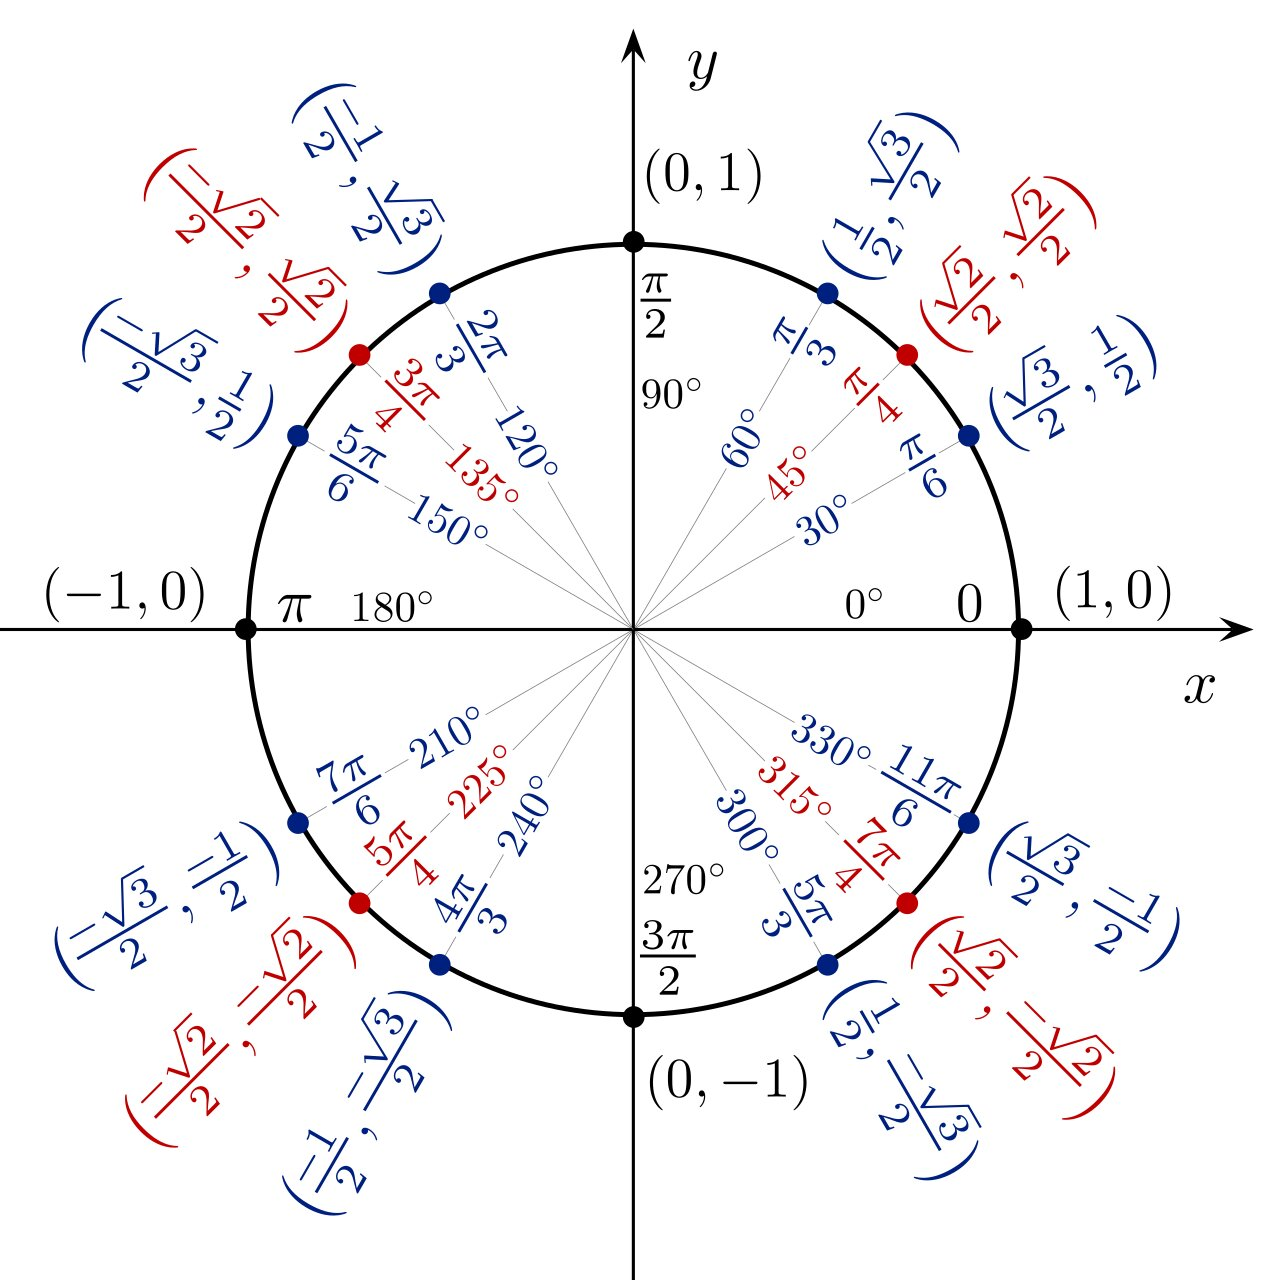
\includegraphics[width=9cm]{unit-circle.jpg}
	        $\cos\theta = x, \ \sin\theta = y, \ \tan\theta = y/x$
		    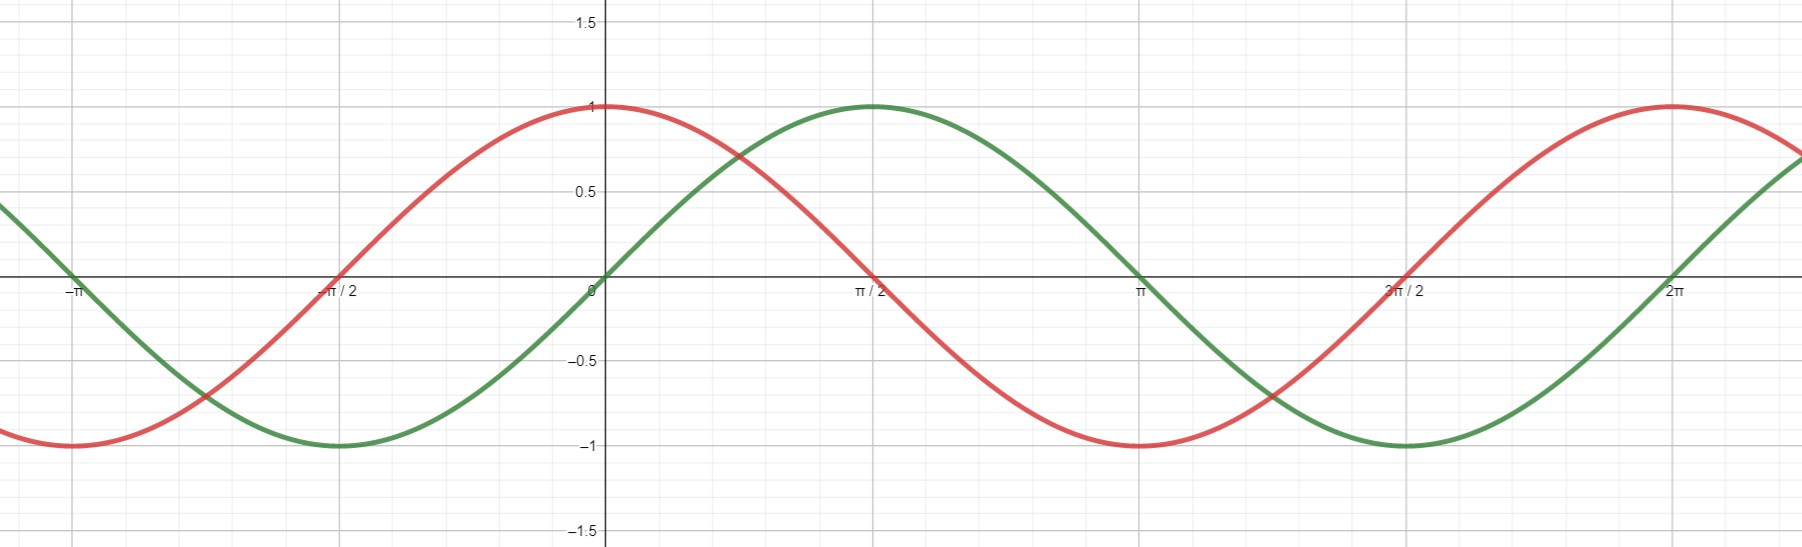
\includegraphics[width=9cm]{cos_sin.jpg}
		    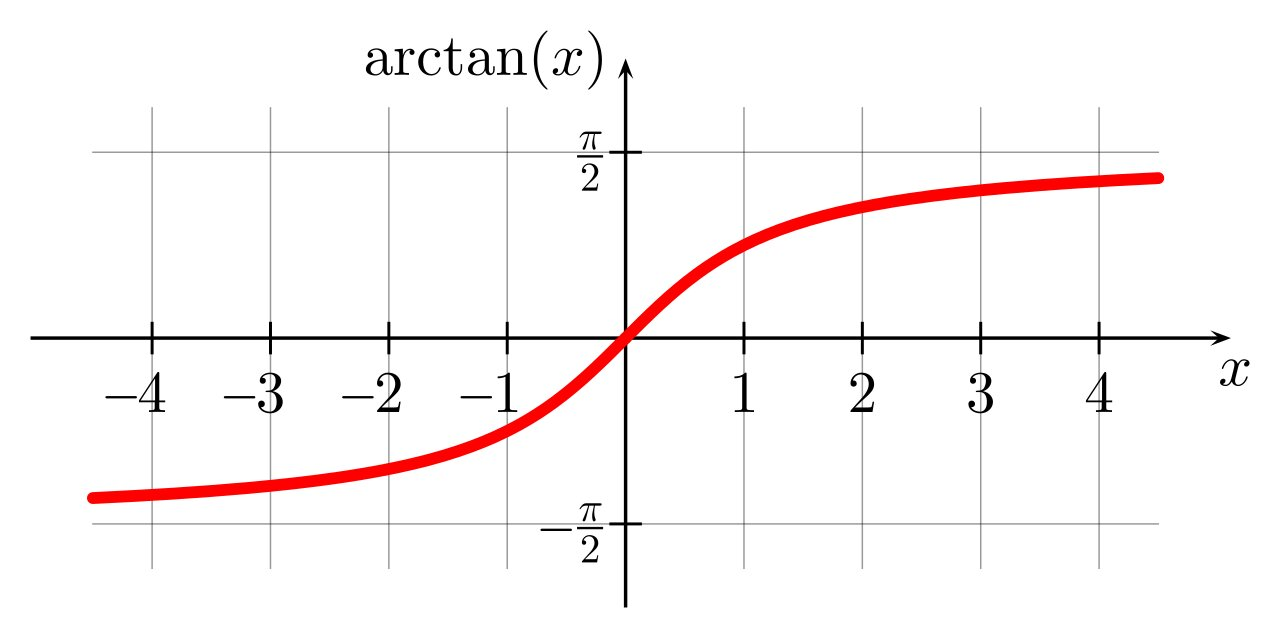
\includegraphics[width=9cm]{arctan.jpg}
		    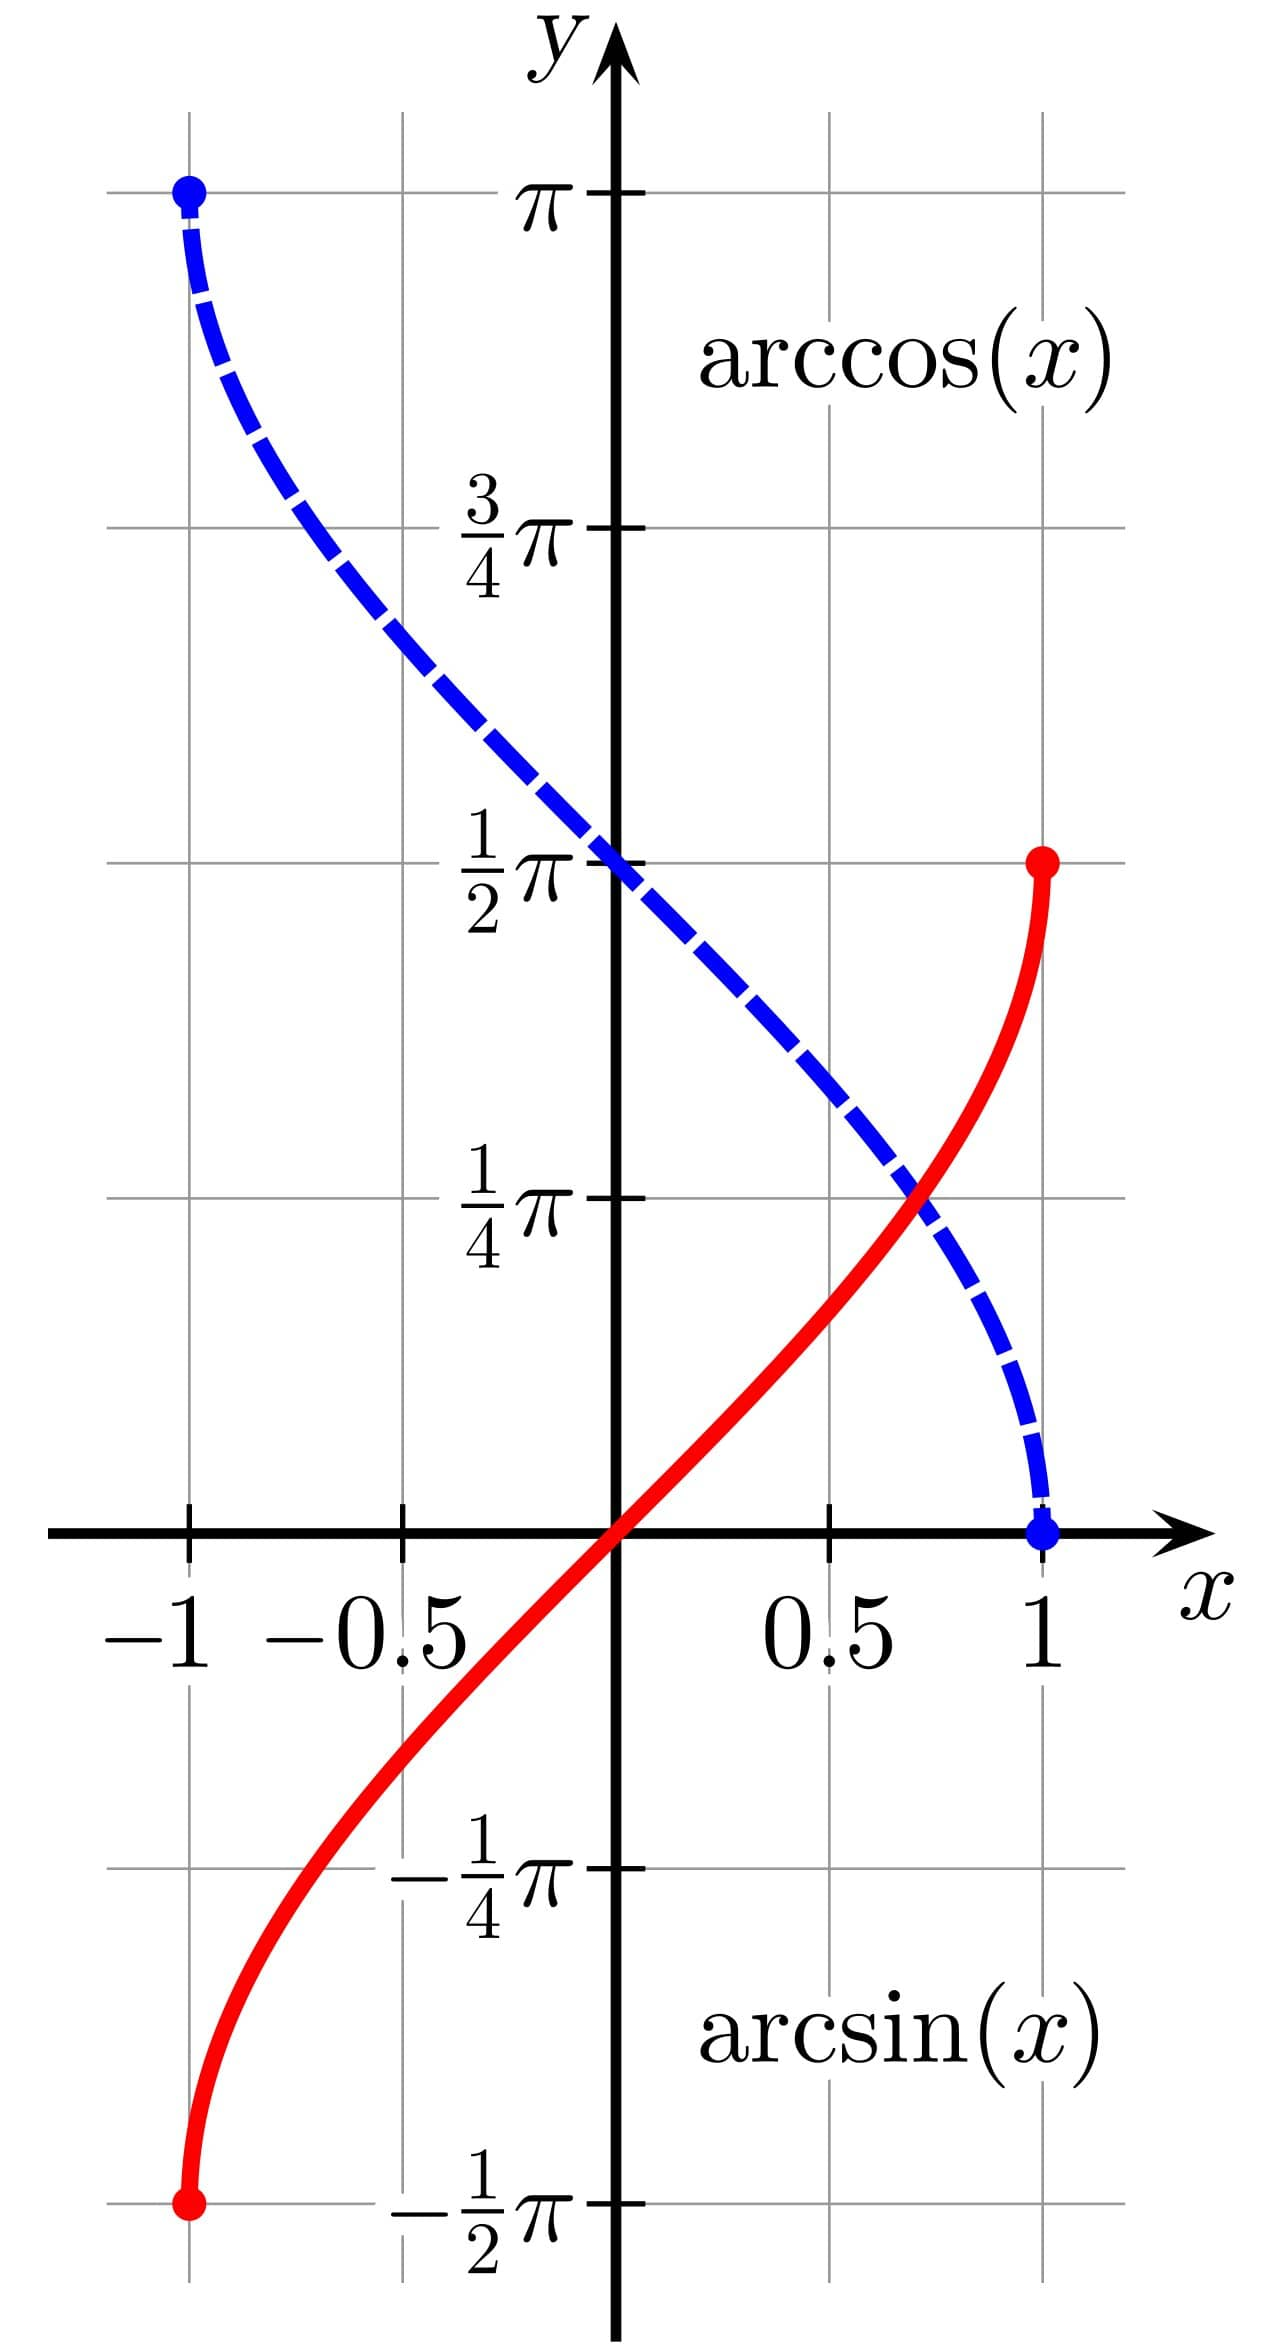
\includegraphics[height=9cm]{arcsin_arccos.jpg}
		 \end{center}
		 \tiny{Quellen: Wikipedia / Geogebra}
		 \normalsize
		 
    \end{multicols*} 
\end{document}